\documentclass[11pt,reqno]{amsart}
\usepackage[T1]{fontenc}
\usepackage{amsmath,amssymb,amsthm,mathtools}
\usepackage{mathrsfs}
\usepackage[margin=1.1in]{geometry}
\usepackage{microtype}
\usepackage{enumitem}
\usepackage{graphicx}
\usepackage{xcolor}
\usepackage[colorlinks=true,linkcolor=blue!55!black,citecolor=teal!60!black,urlcolor=blue!55!black]{hyperref}

\hypersetup{
  pdftitle={Quasi-Stationary Response Geometry: The Perturbation Calculus and Information Geometry of Parametrized Sub-Markovian Generators},
  pdfauthor={Ayush Sarkar},
  pdfkeywords={quasi-stationary distribution; Perron-Frobenius; Metzler matrix; sub-Markovian generator; group inverse; reduced resolvent; analytic perturbation; Fisher information; Fisher-Rao metric; information geometry; invariant subspace; spectral projection; Whitney stratification; saddle-node; identifiability}
}

\theoremstyle{plain}
\newtheorem{theorem}{Theorem}[section]
\newtheorem{proposition}[theorem]{Proposition}
\newtheorem{lemma}[theorem]{Lemma}
\newtheorem{corollary}[theorem]{Corollary}

\theoremstyle{definition}
\newtheorem{definition}[theorem]{Definition}
\newtheorem{example}[theorem]{Example}
\newtheorem{assumption}[theorem]{Assumption}

\theoremstyle{remark}
\newtheorem{remark}[theorem]{Remark}
\newtheorem{notation}[theorem]{Notation}

\newcommand{\R}{\mathbb{R}}             
\newcommand{\C}{\mathbb{C}}              
\newcommand{\Reg}{\Theta_{\mathrm{reg}}} 
\newcommand{\Simp}{\Delta^{\!\circ}}     
\newcommand{\one}{\mathbf{1}}            
\newcommand{\KL}{D_{\mathrm{KL}}}        
\newcommand{\FR}{\mathrm{FR}}       
\newcommand{\abscissa}{\mathfrak{s}}
\newcommand{\dgraph}{\mathcal{D}}
\newcommand{\dd}{\mathrm{d}}

\DeclareMathOperator{\spec}{spec}
\DeclareMathOperator{\rank}{rank}
\DeclareMathOperator{\Imm}{Im}
\DeclareMathOperator{\diag}{diag}
\DeclareMathOperator{\tr}{tr}
\DeclareMathOperator{\Hess}{Hess}

\begin{document}

\title[Quasi-Stationary Response Geometry]{Quasi-Stationary Response Geometry:\\
The Perturbation Calculus and Information Geometry\\ of Parametrized Sub-Markovian Generators}

\author{Ayush Sarkar}
\address{New York University}
\email{as17812@nyu.edu}

\date{\today}

\subjclass[2020]{Primary 15B48, 47A55, 53B12; Secondary 15A18, 62B11, 60J27, 58K05}

\keywords{Quasi-stationary distribution, Perron--Frobenius theory, Metzler matrix,
sub-Markovian generator, group inverse, reduced resolvent, analytic perturbation,
Fisher information, Fisher--Rao metric, information geometry, invariant subspace,
spectral projection, Whitney stratification, saddle--node bifurcation, identifiability.}

\begin{abstract}
Let $\theta\mapsto Q(\theta)$ be a real-analytic family of irreducible Metzler matrices with
nonpositive, not identically vanishing row sums --- the generators of killed (sub-Markovian)
continuous-time Markov chains. The principal spectral datum is the pair $(\Lambda,\nu)$: the magnitude
$\Lambda>0$ of the spectral abscissa (the \emph{decay rate}) and the associated positive left Perron
eigenvector $\nu$, normalized to a probability vector (the \emph{quasi-stationary distribution}, QSD).
We develop a closed first-order response calculus for $(\Lambda,\nu)$ on the irreducible locus, whose
organizing object is the \emph{rate channel}: the decay rate $\Lambda$ is a second response coordinate
with no analogue in the conservative stationary-chain theory, supplying a rank-one term throughout.
Algebraic simplicity and a strict spectral gap are rigid on this locus, giving an invariant-subspace
splitting $\R^{T}=\langle h\rangle\oplus\Imm(Q+\Lambda I)$ with rank-one projection $P=h\nu$ and reduced
resolvent (group inverse) $R=(Q+\Lambda I)^{\#}$; the exact derivatives of $\Lambda$, $\nu$, and $P$ are
a Hellmann--Feynman pairing and a reduced-resolvent action with an explicit normalization correction,
reducing to the classical group-inverse sensitivity calculus of conservative chains in the no-killing
limit $\Lambda\to0$. The QSD map pulls the Fisher--Rao metric of the simplex back to a Fisher
information metric $\mathcal G=J^{\top}\diag(1/\nu)J$ --- the KL Hessian, with null space the
non-identifiable directions --- augmented by a rank-one rate channel adjoining $\log\Lambda$. Under a
self-consistent coupling, a regular branch approaching a simple fold acquires a rank-one $\sigma^{-1}$
response of the datum and a $\sigma^{-2}$ divergence of the pulled-back Fisher metric, gated by an
explicit condition fixing \emph{which} channel --- the QSD law $\nu$ or the rate $\Lambda$ ---
inherits it. The four classical pillars (Perron--Frobenius, Kato/group-inverse perturbation theory,
information geometry, fold theory) are used as tools; what is new is the killed-case calculus organized
around the rate channel, the channel split between $\dd\nu$ and $\dd\Lambda$, the which-channel
fold-transport bookkeeping with its observable-coupling condition, and an exactly $e$-flat,
properly-non-uniform realizability witness.

The calculus transports to the operator setting: under a Foster--Lyapunov drift the principal datum,
its fold amplification, and the $\Lambda\to0$ recovery lift to non-compact state spaces as a
\emph{rigorous corollary of cited QSD theory}, discharged on an exactly-solvable countable
birth--death-with-killing instance, with the diffusion case at sketch level. The finite-$N$ fluctuation
layer and the resulting fold-sensing Cram\'er--Rao floor are developed in a companion
paper~\cite{SarkarFoldSensing}, of which this paper is the deterministic core.
\end{abstract}

\maketitle

\newpage
\tableofcontents
\newpage

\section{Introduction}\label{sec:intro}


\subsection{The object of study}
Fix a finite set $T$ with $|T|=n\ge 2$. A real $n\times n$ matrix $Q$ is
\emph{Metzler} (or \emph{essentially nonnegative}) if its off-diagonal entries are
nonnegative, $Q_{ss'}\ge 0$ for $s\neq s'$. Such matrices are exactly the
infinitesimal generators of nonnegative one-parameter semigroups
$e^{tQ}\ge 0$, and a Metzler matrix with $Q\one\le 0$ is the generator of a
\emph{sub-Markovian} (killed, sub-conservative) continuous-time Markov chain on
$T$: the row defect $q:=-Q\one\ge 0$ is the vector of killing rates, and
$Q\one=-q\le0$ records that probability mass may leak out of $T$ into an
adjoined absorbing cemetery. When $q\equiv 0$ the matrix is a conservative
generator and the long-run object is a stationary distribution; when $q\not\equiv
0$ the only stationary distribution is the point mass at the cemetery, and the
relevant long-run object is instead the \emph{quasi-stationary distribution}.

Concretely, write $\abscissa(Q):=\max\{\Re\mu\mid\mu\in\spec(Q)\}$ for the
\emph{spectral abscissa}. We will see that for an irreducible Metzler $Q$ with
$q\not\equiv 0$ the abscissa is a real, algebraically simple, strictly dominant
eigenvalue $\abscissa(Q)=-\Lambda$ with $\Lambda>0$, carrying strictly positive
left and right eigenvectors $\nu$ and $h$. Normalizing $\nu\one=1$ makes $\nu$ a
probability vector. The pair
\[
\bigl(\Lambda,\ \nu\bigr)\in\R_{>0}\times\Simp,
\qquad
\Simp:=\Bigl\{p\in\R^{T}_{>0}\Bigm|\textstyle\sum_{s}p_s=1\Bigr\},
\]
is the \emph{principal spectral datum} of $Q$. Probabilistically, $\Lambda$ is the
exponential decay rate of survival, $\mathbb P(\text{not yet killed at time }t)
\asymp e^{-\Lambda t}$, with $1/\Lambda$ the mean time to absorption from $\nu$,
and $\nu$ is the Yaglom limit, the law of the state conditioned on survival; see
Darroch and Seneta~\cite{DarrochSeneta1967} for the finite case and
\cite{MeleardVillemonais2012,ColletMartinezSanMartin2013,vanDoornPollett2013} for
the general theory. None of the geometry below requires the probabilistic
reading: it is a statement about the principal spectral datum of an essentially
nonnegative matrix, and applies equally to any setting in which such matrices
arise parametrically.

\subsection{The question}
Let $\Theta$ be a (finite-dimensional, real-analytic) parameter manifold and
$\theta\mapsto Q(\theta)$ a real-analytic family of irreducible Metzler
sub-generators. As $\theta$ varies, the principal datum
$\theta\mapsto(\Lambda(\theta),\nu(\theta))$ traces a curve, surface, or
higher-dimensional locus in $\R_{>0}\times\Simp$. We ask:

\begin{enumerate}[label=\textup{(Q\arabic*)},leftmargin=3.2em]
\item\label{q:reg} \emph{Regularity.} Where is $(\Lambda,\nu)$ analytic in
$\theta$, and what obstructs analyticity?
\item\label{q:resp} \emph{Response.} What are the exact first-order derivatives
$\dd\Lambda$ and $\dd\nu$, and what linear-algebraic objects carry them?
\item\label{q:geom} \emph{Geometry.} What is the natural Riemannian/statistical
geometry induced on $\Theta$ by the map $\theta\mapsto(\Lambda(\theta),\nu(\theta))$,
and what do its degeneracies mean?
\item\label{q:strat} \emph{Stratification.} When the operative parameter is itself
constrained by an implicit (self-consistent) relation, how does the geometry
behave near the folds of that relation, and how do the folds partition $\Theta$?
\end{enumerate}

\subsection{Results and organization}
The paper answers~\ref{q:reg}--\ref{q:strat} by assembling four classical
theories into a single response calculus. The lead novelty is small and stated as
such: a \emph{rate channel}, the second response coordinate $\Lambda$, which has no
analogue in the conservative stationary-chain theory and supplies the rank-one
terms throughout (\S\ref{sec:perturbation}, \S\ref{sec:infogeom}). Around it the
fold result of \S\ref{sec:manifold} (Theorem~\ref{thm:fold}) is the classical
implicit-function blow-up at a simple fold, transported through the chain rule into
the $(\Lambda,\nu)$ channels: when an observable of the quasi-stationary datum
feeds back into the generator, the closed-loop response of $(\Lambda,\nu)$ inherits
the rank-one divergence of the self-consistency branch derivative --- at rate
$\sigma^{-1}$ for the datum's response and $\sigma^{-2}$ for the pulled-back information
metric. Its contribution is not the blow-up itself, which is the implicit function
theorem near a fold, but the bookkeeping of \emph{which channel sees it}: the QSD
channel inherits the divergence \emph{precisely when} $\partial_u\nu$ couples to the
fold direction, and the rate channel \emph{precisely when} $\partial_u\Lambda$ does.
The sections before it build the machinery this theorem consumes; the sections
after it verify the calculus in closed form.

To draw the boundary between new and assembled at the outset: the
\emph{assembled} ingredients --- Perron--Frobenius theory, Kato perturbation
theory, the group-inverse sensitivity calculus of stationary chains, classical
information geometry, and the singularity theory of fold maps --- are classical
and are used here as tools. What we claim as \emph{new} is (a)~the killed-case
response calculus itself: the group-inverse perturbation formulas for the
principal datum of a properly killed generator, organized around the second
response coordinate $\Lambda$ (the rate channel), which has no analogue in the
conservative theory and reduces to it as $\Lambda\to0$; and (b)~the fold
amplification theorem with its observable-coupling condition, which transports
the implicit-function blow-up through the QSD and rate channels and identifies
exactly when each channel sees it. The information-geometry pillar adds (c)~an exactly
$e$-flat killed-generator family with properly non-uniform killing and a response image
of dimension $\ge2$ (Example~\ref{ex:eflat-nonuniform}, Proposition~\ref{prop:eflat-nonuniform}),
showing realizability of the flat case by explicit construction. The remaining named statements
--- the rigidity of simplicity, the channel split, the foliation --- are short
consequences recorded because later sections consume them, not claims of
novelty. The finite-$N$ fluctuation layer and the fold-sensing Cram\'er--Rao floor,
which carry the $\sigma^{-2}$ amplification of this paper into a statistical
resolution limit, are developed in the companion paper~\cite{SarkarFoldSensing}.

\smallskip
The contributions of the paper, in the order they appear, are the following.
\begin{itemize}[leftmargin=1.6em]
\item A closed first-order \emph{response calculus} for the principal datum
$(\Lambda,\nu)$ of a killed (sub-Markovian) generator, organized around the rate
channel $\Lambda$ and the reduced resolvent (group inverse) $R$, reducing to the
classical stationary-chain sensitivity theory as $\Lambda\to0$
(\S\ref{sec:perturbation}).
\item The pulled-back \emph{information geometry} of the QSD map. That
$\mathcal G=J^\top\diag(1/\nu)J$ is the Fisher information and the KL Hessian is
textbook; the new ingredient is the one-line \emph{rate-channel augmentation}
adjoining $\log\Lambda$ (Definition~\ref{def:augmented}), together with the
non-identifiability foliation cut out by the kernel
(\S\ref{sec:infogeom}--\S\ref{sec:manifold}).
\item The \emph{fold transport} theorem: the classical implicit-function blow-up at
a simple fold, transported through the chain rule into a rank-one singularity --- at rate
$\sigma^{-1}$ for the closed-loop datum's response and $\sigma^{-2}$ for the information
metric --- with the contribution being the which-channel-sees-it bookkeeping gated by
an explicit observable-coupling condition (\S\ref{sec:manifold}).
\item An \emph{exactly $e$-flat non-uniform family} (\S\ref{sec:infogeom}): a tilted-reset
killed generator whose QSD response image is an exponential family of dimension $\ge2$
\emph{with} properly non-uniform killing ($h\neq\one$, active normalization correction),
exercising the killed-case information geometry in the flat, multi-dimensional regime
(Example~\ref{ex:eflat-nonuniform}).
\item A record of how the calculus \emph{transports} to the operator setting
(\S\ref{sec:infinite-dim}): under a Foster--Lyapunov drift, QSD existence, the
amplification, the group-inverse calculus, and the $\Lambda\to0$ recovery lift to
non-compact state spaces. This is an \emph{assembly} of cited theorems, not a new one ---
a rigorous corollary for the countable case, anchored on a worked exactly-solvable
instance (Poisson QSD, $\Lambda=\tfrac16$ in the calibrated case), with the diffusion case
at sketch level.
\end{itemize}
The finite-$N$ fluctuation layer and the fold-sensing resolution floor (a Cram\'er--Rao
bound unifying the $\sigma^{-2}$ amplification with the finite-$N$ width) are the subject
of the companion paper~\cite{SarkarFoldSensing}.

\smallskip
\noindent\textbf{Spectral foundation (\S\ref{sec:spectral}).}
Theorem~\ref{thm:pf} establishes that the principal datum is well defined,
real-analytic on the irreducible locus $\Reg$, and carried by a simple, strictly
dominant eigenvalue. Proposition~\ref{thm:rigidity} records the accompanying
rigidity, answering~\ref{q:reg}: simplicity of the Perron eigenvalue cannot fail
while irreducibility holds, so the spectral singular set is confined to
$\partial\Reg$ --- a short consequence of Perron--Frobenius positivity and the
continuity of spectra, stated explicitly because the perturbation and geometry
sections consume it.

\smallskip
\noindent\textbf{Invariant subspaces and the reduced resolvent (\S\ref{sec:invariant}).}
Simplicity gives a canonical splitting $\R^{T}=\Imm P\oplus\ker P$ into
$Q$-invariant subspaces, with $P=h\nu$ the Riesz projection and
$R=(Q+\Lambda I)^{\#}$ the group inverse on the complement
(Proposition~\ref{prop:splitting}). This is the algebraic substrate for the
response calculus.

\smallskip
\noindent\textbf{Response calculus (\S\ref{sec:perturbation}).}
Answering~\ref{q:resp}, Theorem~\ref{thm:response} gives the projection
derivative $\dd P=-(R\,\dd Q\,P+P\,\dd Q\,R)$, the eigenvalue derivative
$\dd\Lambda=-\nu\,(\dd Q)\,h$ (Hellmann--Feynman), and the eigenvector derivative
$\dd\nu=-\nu\,(\dd Q)\,R+\bigl(\nu\,(\dd Q)\,R\,\one\bigr)\nu$. We give the
second-order curvature of $\Lambda$ (Proposition~\ref{prop:second-order}) and show
the entire calculus reduces, as $\Lambda\to 0$, to the group-inverse / fundamental-matrix
sensitivity theory of stationary Markov chains
(Schweitzer~\cite{Schweitzer1968}, Meyer~\cite{Meyer1975}, Golub--Meyer~\cite{GolubMeyer1986}),
with the correct sign (Theorem~\ref{thm:conservative-limit}).

\smallskip
\noindent\textbf{Information geometry (\S\ref{sec:infogeom}).}
Answering~\ref{q:geom}, Theorem~\ref{thm:fisher} shows that the QSD map pulls the
Fisher--Rao metric of $\Simp$ back to the Fisher information metric
$\mathcal G=J^{\top}\diag(1/\nu)\,J$ of the family $\{\nu(\theta)\}$, equal to the
Hessian of Kullback--Leibler divergence, with $\ker\mathcal G=\ker\dd\nu$
identifying the non-identifiable directions. The identity $\mathcal G=$ Fisher $=$
KL Hessian is textbook (it holds for any smooth statistical family); what is specific
to the killed-generator setting is the second response coordinate, so the one new
line here is the rank-one \emph{rate-channel augmentation}
$\mathcal G^{\oplus}=\mathcal G+w\,\dd(\log\Lambda)\otimes
\dd(\log\Lambda)$ (Definition~\ref{def:augmented}), which adjoins $\log\Lambda$ to
the QSD observable. The construction is coordinate-free
(Proposition~\ref{prop:coordinate-free}). We recall that the ambient
simplex is dually flat, while the response image inherits the Fisher geometry on
constant-rank strata; exact Pythagorean projection identities require additional
flatness hypotheses (Remark~\ref{rem:dually-flat}), illustrated by the explicit
$e$-flat QSD family of Example~\ref{ex:eflat}.

\smallskip
\noindent\textbf{Response manifold and stratification (\S\ref{sec:manifold}).}
Answering~\ref{q:strat}, Theorem~\ref{thm:rank} exhibits the response image as a
low-dimensional immersed submanifold of $\Simp$ on each constant-rank stratum,
foliated by non-identifiability leaves. Theorem~\ref{thm:fold} treats self-consistent
coupling. The mechanism is classical --- along a regular branch approaching a simple
fold of the self-consistency relation, the implicit branch derivative
$\partial_\theta u^*=-(\partial_u F)^{-1}\partial_\theta F$ has a rank-one $\sigma^{-1}$
singularity by the implicit function theorem; the chain rule then transports this into
the closed-loop datum. The contribution is the \emph{which-channel} bookkeeping: the
QSD information metric inherits a rank-one divergence precisely when $\partial_u\nu$
couples to the fold direction, the rate channel precisely when $\partial_u\Lambda$ does
(Example~\ref{ex:scalarfold} shows the blow-up is exactly the elementary
$\dd\sqrt\theta/\dd\theta$).
Remark~\ref{rem:stratification} interprets the discriminant, under properness and
Thom--Boardman genericity assumptions, as giving a Whitney-stratified family of
regimes; Remark~\ref{rem:slowing} points to the corresponding small-noise scaling
heuristics (recorded for orientation only).

\smallskip
\noindent\textbf{Examples (\S\ref{sec:eflat}, \S\ref{sec:fold-divergence},
\S\ref{sec:examples}).}
Example~\ref{ex:eflat} constructs an exactly $e$-flat QSD response family, showing
that the classical information-projection geometry is realizable inside the
killed-generator framework (in the uniform-killing subcase);
Example~\ref{ex:nonuniform} complements it with a properly non-uniform family
($h\neq\one$) whose non-identifiability foliation, rank-one metric, and channel
split are global, affine, and in closed form; and
Example~\ref{ex:eflat-nonuniform} combines the two regimes in a \emph{tilted reset},
realizing exact $e$-flatness \emph{together with} properly non-uniform killing and a
response image of dimension $\ge2$. Example~\ref{ex:scalarfold} gives a closed-form scalar
fold verifying the $\sigma^{-2}$ metric blow-up and the necessity of the
observable-coupling condition. Section~\ref{sec:examples} works the two-state
killed chain in closed form, verifies the response formulas and the sign, exhibits
the conservative limit, proves the structural \emph{channel split}
$\ker\dd\nu\neq\ker\dd\Lambda$ via a scaling gauge
(Proposition~\ref{prop:channel-split}), and gives a self-consistent three-state
example realizing a fold numerically.

All displayed first- and second-order formulas were verified numerically against
finite differences on randomly generated irreducible Metzler families; the
verification is described in Remark~\ref{rem:numerics}.

\subsection{Relation to the literature}
The four pillars are individually classical. Perron--Frobenius theory for
nonnegative and Metzler matrices is in
Berman--Plemmons~\cite{BermanPlemmons1994},
Horn--Johnson~\cite{HornJohnson2013}, and Seneta~\cite{Seneta2006}. Analytic
perturbation of a simple isolated eigenvalue is Kato~\cite{Kato1995}; the
derivative of the Perron root of an essentially nonnegative matrix, expressed
through the group inverse of the associated $M$-matrix, is
Deutsch--Neumann~\cite{DeutschNeumann1984}; and the group-inverse formulation of
finite-Markov-chain sensitivity is due to
Schweitzer~\cite{Schweitzer1968}, Meyer~\cite{Meyer1975},
Campbell--Meyer~\cite{CampbellMeyer2009}, Golub--Meyer~\cite{GolubMeyer1986},
and Cho--Meyer~\cite{ChoMeyer2001}. Information geometry --- the Fisher--Rao
metric, the $\pm1$ connections, dual flatness, and the projection theorems --- is
\v{C}encov~\cite{Cencov1982}, Amari--Nagaoka~\cite{AmariNagaoka2000},
Amari~\cite{Amari2016}, and Ay--Jost--L\^e--Schwachh\"ofer~\cite{Ay2017}. Whitney
stratification and the singularity theory of fold maps are
Whitney~\cite{Whitney1965}, Mather~\cite{Mather2012}, Thom~\cite{Thom1969},
Golubitsky--Guillemin~\cite{GolubitskyGuillemin1973},
Arnold~\cite{Arnold1992}, and Goresky--MacPherson~\cite{GoreskyMacPherson1988};
the relevant bifurcation normal forms are in Kuznetsov~\cite{Kuznetsov2004} and
Guckenheimer--Holmes~\cite{GuckenheimerHolmes1983}, and the small-noise scaling in
van Kampen~\cite{vanKampen2007}.

The contribution of the present paper is the synthesis: we treat the principal
spectral datum of a \emph{killed} (sub-Markovian) generator as a map into
$\R_{>0}\times\Simp$ and show that its differential geometry is governed jointly
by the group-inverse perturbation calculus and the pulled-back Fisher--Rao
metric, with the non-identifiability foliation and the fold stratification as the
manifold-theoretic backbone. The conservative theory of
\cite{Schweitzer1968,Meyer1975} is the boundary case $\Lambda=0$, and the second,
genuinely new response coordinate $\Lambda$ supplies the rank-one terms
throughout. The motivating instance --- the response of a metastable population
model to parameter interventions --- is described in
\S\ref{sec:applications}, but the theory is stated and proved with no reference to
any particular model. Concretely, the individual ingredients are classical; the four parts claimed as
new --- the killed-case group-inverse response calculus organized around the rate channel, the channel
split, the fold-transport which-channel bookkeeping, and the $e$-flat properly-non-uniform
realizability witness --- are the (a)--(d) stated above (\S\ref{sec:intro}), here positioned against the
literature rather than re-enumerated; the remaining named statements (Perron rigidity, the
non-identifiability foliation) are recorded consequences. The paper may also be read
as the methods companion to the modeling application of \S\ref{sec:applications},
from which the questions~\ref{q:reg}--\ref{q:strat} were abstracted.

Closest to the present perturbation analysis is the work of Rudolf and
Wang~\cite{RudolfWang2021} on the stability of quasi-stationary distributions of
killed Markov processes, which gives $L^1$-norm bounds on the QSD response to
bounded generator perturbations in a self-adjoint operator setting; our concern is
complementary --- exact first-order derivatives of the principal datum and the
information geometry they induce, in the finite irreducible Metzler setting. An
information-geometric treatment of a different Markov-chain functional --- the
class-conditional hitting-time laws of an absorbing chain under a log-linear edge
model $A_{ij}(\theta)=A_{ij}^{(0)}e^{\theta^{\top}\phi_{ij}}$ --- was recently given
by Kimura~\cite{AbsIG2026}, who computes the (observed) Fisher information of the
hitting-time law, finds it rank-one per seed node, and reads its null space as the
non-identifiable edge directions. The structural parallel is real, and it is at the
level of the \emph{shared apparatus}: a pulled-back Fisher form that is rank-one with
a non-identifiability foliation cut out by its kernel. We claim no novelty for that
apparatus --- it is classical information geometry, parallel on both sides. The
genuine difference is the \emph{object} being parametrized. A first-passage law
carries no rate channel; the present paper parametrizes the principal spectral datum
$(\Lambda,\nu)$ of a \emph{killed} generator, whose decay rate $\Lambda$ is a second
response coordinate with no analogue in a hitting-time functional (which has no
principal eigenvalue datum to differentiate). The increment claimed here is therefore
precisely the Perron/resolvent perturbation calculus this datum requires: the
group-inverse response formulas of Theorem~\ref{thm:response}, the rate channel and
channel split (Proposition~\ref{prop:channel-split}), Perron rigidity on the
irreducible killed locus (Proposition~\ref{thm:rigidity}), and the self-consistent
fold amplification of Theorem~\ref{thm:fold} (with the saddle--node scaling heuristics
of Remark~\ref{rem:slowing}) --- none of which \cite{AbsIG2026} carries, because a
first-passage functional has no rate channel to begin with. The non-identifiability
geometry is also the ``sloppy model'' / model-manifold
phenomenon~\cite{Transtrum2015,ModelManifoldGeom} of the parameter-estimation
literature.

The infinite-dimensional extension of \S\ref{sec:infinite-dim} draws on
further classical lines: the QSD theory rests on the Champagnat--Villemonais Lyapunov
criterion for non-compact killed processes~\cite{ChampagnatVillemonais2016,%
ChampagnatVillemonais2017}, on Krein--Rutman positivity in a weighted
cone~\cite{KreinRutman1948}, and on Meyn--Tweedie Foster--Lyapunov
theory~\cite{MeynTweedie2009}. The companion paper~\cite{SarkarFoldSensing}, which
carries the fold amplification into the finite-$N$ and statistical regime, draws in
addition on the metastability/critical-slowing-down literature of
Berglund--Gentz~\cite{BerglundGentz2006} and van Kampen~\cite{vanKampen2007}. The motivating application --- a metastable
behavioral population leaking to an absorbing death state --- is in the spirit of
the opioid-epidemic and post-release-mortality modeling of
Bukten et al.~\cite{Bukten2017}, though, as
emphasized throughout, the theory is stated and proved with no reference to any
particular model.

\smallskip
\noindent\textbf{Scope of the results.}
The core results (\S\S\ref{sec:spectral}--\ref{sec:manifold}) are finite-dimensional and are stated on
the regular locus of irreducible, properly killed Metzler sub-generators; their operator-theoretic
transport to countable and diffusion state spaces, under cited hypotheses, is \S\ref{sec:infinite-dim}
(a rigorous corollary of cited QSD theory for the countable case, a sketch for the diffusion case). On
this locus the Perron datum is analytic and the principal eigenvalue cannot coalesce with the rest of
the spectrum; spectral singularities therefore occur only at the boundary, where
irreducibility or proper killing fails. The fold results of \S\ref{sec:manifold}
concern a different source of singular behavior: an implicit self-consistency
relation $F(\theta,u)=0$, whose regular branches may approach a fold of the
projection $\mathcal S\to\Theta$ --- not a coalescence of the Perron eigenvalue. The
Whitney-stratified-regime language and the small-noise fold exponents are used only
under the additional genericity/properness or stochastic normal-form assumptions
stated there.

\smallskip
\noindent\textbf{Reader's guide (proof dependencies).}
Sections~\ref{sec:spectral}--\ref{sec:examples} are the \emph{proved finite-dimensional core}: the
Perron--Frobenius foundation (\S\ref{sec:spectral}), the invariant-subspace splitting and reduced
resolvent (\S\ref{sec:invariant}), the first-order response calculus with its conservative limit
(\S\ref{sec:perturbation}), the pulled-back information geometry (\S\ref{sec:infogeom}), the response
manifold and fold transport (\S\ref{sec:manifold}), and the worked examples (\S\ref{sec:examples}).
Every theorem there is proved in full, and the displayed formulas are independently checked against
finite differences (Remark~\ref{rem:numerics}). Section~\ref{sec:infinite-dim} is operator-theoretic
\emph{transport} under cited hypotheses: the countable case is a rigorous corollary of cited QSD theory
discharged on an explicit exactly-solvable instance, the diffusion case is at the level of a sketch.
Remarks~\ref{rem:stratification}--\ref{rem:slowing} (Whitney stratification, small-noise scalings) are
interpretive, recorded under the additional genericity/stochastic hypotheses stated there. The
finite-$N$ fluctuation layer and the Cram\'er--Rao fold-sensing floor are the subject of the companion
paper~\cite{SarkarFoldSensing}; the present paper is self-contained without them.


\section{Principal spectral data of irreducible sub-generators}\label{sec:spectral}


\begin{notation}
Vectors are columns; $\one\in\R^{T}$ is the all-ones vector; row vectors are
written with a left action, e.g.\ $\nu Q$. For a Metzler matrix $Q$ we write
$q:=-Q\one$ for the \emph{killing vector}. The directed graph $\dgraph(Q)$ has
vertex set $T$ and an edge $s\to s'$ whenever $s\neq s'$ and $Q_{ss'}>0$; $Q$ is
\emph{irreducible} when $\dgraph(Q)$ is strongly connected. We write $\spec(Q)$
for the spectrum and $\abscissa(Q)=\max\{\Re\mu\mid\mu\in\spec(Q)\}$ for the spectral
abscissa.
\end{notation}

\begin{definition}[Sub-generator]\label{def:subgen}
A matrix $Q\in\R^{T\times T}$ is a \emph{sub-generator} if it is Metzler
($Q_{ss'}\ge0$ for $s\neq s'$) and sub-conservative ($Q\one\le 0$). It is
\emph{properly killed} if $q=-Q\one\neq 0$, and \emph{conservative} if $q=0$. We
denote by $\mathcal M_{\mathrm{irr}}(T)$ the set of irreducible, properly killed
sub-generators on $T$.
\end{definition}

The next theorem is the Perron--Frobenius foundation. It is a routine consequence
of the classical theorem applied to a diagonal shift, but we give the full
argument because the strict dominance in \emph{real part} (not merely modulus) and
the positivity of $\Lambda$ are exactly the hypotheses the perturbation and
geometry sections consume.

\begin{theorem}[Principal datum]\label{thm:pf}
Let $Q\in\mathcal M_{\mathrm{irr}}(T)$. Then:
\begin{enumerate}[label=\textup{(\roman*)}]
\item The spectral abscissa $\abscissa(Q)$ is an eigenvalue of $Q$; it is real,
algebraically simple, and \emph{strictly dominant}: $\Re\mu<\abscissa(Q)$ for every
$\mu\in\spec(Q)\setminus\{\abscissa(Q)\}$.
\item The corresponding left and right eigenvectors $\nu,h$ may be chosen strictly
positive, and are unique up to positive scaling. Normalize $\nu\one=1$ and
$\nu h=1$.
\item Writing $\abscissa(Q)=-\Lambda$, one has $\Lambda>0$ and the identity
$\Lambda=\nu q=-\nu Q\one$.
\item \textup{(Converse Perron characterization.)} $\abscissa(Q)$ is the unique
eigenvalue of $Q$ admitting a strictly positive right eigenvector, and the unique
eigenvalue admitting a strictly positive left eigenvector. Equivalently: if
$Qh'=\lambda h'$ with $h'>0$, or $\nu'Q=\lambda\nu'$ with $\nu'>0$, then
$\lambda=\abscissa(Q)$.
\end{enumerate}
\end{theorem}

\begin{proof}
Choose a scalar $c>\max_{s}|Q_{ss}|$ and set $M:=Q+cI$. Then $M\ge0$ entrywise:
off-diagonals are those of $Q$ (nonnegative), and diagonals are $Q_{ss}+c>0$.
Since a diagonal shift does not change off-diagonal support, $\dgraph(M)=\dgraph(Q)$
is strongly connected, so $M$ is an irreducible nonnegative matrix. By the
Perron--Frobenius theorem~\cite[Thm.~8.4.4]{HornJohnson2013} its spectral radius
$r:=\rho(M)>0$ is an algebraically simple eigenvalue with strictly positive left
and right eigenvectors $\nu,h$, and every $\mu_M\in\spec(M)$ satisfies $|\mu_M|\le
r$.

Because $\spec(Q)=\spec(M)-c$, the value $\abscissa(Q)=r-c=:-\Lambda$ is an
algebraically simple eigenvalue of $Q$ with the same eigenvectors $\nu,h>0$,
proving the eigenvector claims in (ii). For strict dominance, let
$\mu=\mu_M-c\in\spec(Q)$ with $\mu\neq-\Lambda$. Then
$\Re\mu=\Re\mu_M-c\le|\mu_M|-c\le r-c=-\Lambda$. Equality throughout forces
$|\mu_M|=r$ and $\Re\mu_M=|\mu_M|$, i.e.\ $\mu_M$ real and nonnegative with modulus
$r$, hence $\mu_M=r$ and $\mu=-\Lambda$, a contradiction. Thus
$\Re\mu<-\Lambda=\abscissa(Q)$, proving (i).

Finally, left-multiply $Q\one=-q$ by the positive row vector $\nu$:
$\nu Q\one=-\nu q$. But $\nu Q=-\Lambda\nu$, so $\nu Q\one=-\Lambda(\nu\one)$.
Hence $\Lambda(\nu\one)=\nu q$. Since $\nu>0$, $q\ge0$, and $q\neq0$, the right
side is strictly positive, so $\Lambda>0$; with $\nu\one=1$ we get $\Lambda=\nu q$,
which is (iii).

For (iv), keep $M=Q+cI\ge0$ irreducible as above. By Perron--Frobenius the only
eigenvalue of $M$ possessing a nonnegative (hence, by irreducibility, strictly
positive) eigenvector is the Perron root $\rho(M)=r$. If $Qh'=\lambda h'$ with
$h'>0$, then $Mh'=(\lambda+c)h'$, so $\lambda+c=r$, i.e.\ $\lambda=r-c=\abscissa(Q)$.
Applying the same to $Q^{\top}$ (also irreducible Metzler, with
$\abscissa(Q^{\top})=\abscissa(Q)$) gives the left-eigenvector statement, since a
strictly positive left eigenvector of $Q$ is a strictly positive right eigenvector
of $Q^{\top}$.
\end{proof}

\begin{definition}[QSD map]\label{def:qsd-map}
For $Q\in\mathcal M_{\mathrm{irr}}(T)$ we call $\nu\in\Simp$ the
\emph{quasi-stationary distribution} and $\Lambda>0$ the \emph{decay rate}. For a
family $\theta\mapsto Q(\theta)$ we call
\[
\Phi\colon\Reg\longrightarrow\Simp,\qquad \Phi(\theta):=\nu(\theta),
\]
the \emph{QSD map}, and $\theta\mapsto\Lambda(\theta)$ the \emph{decay-rate
function}, where $\Reg:=\{\theta\mid Q(\theta)\in\mathcal M_{\mathrm{irr}}(T)\}$ is the
\emph{regular} (irreducible, properly killed) locus.
\end{definition}

\begin{remark}[Uniform versus non-uniform killing]\label{rem:uniform-killing}
In the conservative case ($q=0$), the principal eigenvalue is $0$, the right Perron
eigenvector is $h=\one$, and the principal datum reduces to the stationary
distribution $\nu=\pi$. Proper killing introduces a positive decay rate
($\Lambda>0$), but it does not by itself force $h\neq\one$. Indeed,
\[
h=\one
\quad\Longleftrightarrow\quad
Q\one=-\Lambda\one
\quad\Longleftrightarrow\quad
q=\Lambda\one,
\]
so the right Perron eigenvector remains constant exactly when killing is uniform
across states. In that case the killed chain is a conservative chain thinned by an
independent exponential clock: the QSD is the stationary law of $(Q+\Lambda I)$,
while $\Lambda$ records the uniform survival rate.
The genuinely new eigenvector geometry appears when the killing is non-uniform.
Then $h\neq\one$, the Perron line is no longer the constant direction, and the
normalization geometry in the response formulas separates from the conservative
stationary-distribution calculus. Thus the killed theory contains both a
uniform-killing subcase, where the rate channel is present but decoupled from the
QSD eigenvector geometry, and a non-uniform-killing case, where $h\neq\one$ and the
normalization correction $c_j$ is no longer identically zero in general.
\end{remark}

We now record the answer to~\ref{q:reg}. Real-analyticity is Kato's theorem for a
simple isolated eigenvalue; we add the observation --- a short consequence of
Theorem~\ref{thm:pf} and the continuity of spectra, recorded because everything
downstream consumes it --- that on $\Reg$ the eigenvalue is never non-simple, so
there is no interior obstruction.

\begin{proposition}[Analyticity and rigidity]\label{thm:rigidity}
Let $\theta\mapsto Q(\theta)$ be real-analytic on an open set $\Theta$ and valued in
the cone of Metzler sub-generators (each $Q(\theta)$ is Metzler with
$Q(\theta)\one\le 0$), and let $\Reg\subseteq\Theta$ be the regular locus. Then
$\Reg$ is open and:
\begin{enumerate}[label=\textup{(\roman*)}]
\item $\Reg\ni\theta\mapsto\bigl(\Lambda(\theta),\nu(\theta),h(\theta)\bigr)$ is
real-analytic, and so are the spectral projection $P(\theta)=h(\theta)\nu(\theta)$
and the group inverse $R(\theta)=(Q(\theta)+\Lambda(\theta)I)^{\#}$ of
\S\ref{sec:invariant}.
\item \textup{(Rigidity.)} For every $\theta\in\Reg$ the Perron eigenvalue
$-\Lambda(\theta)$ is algebraically simple and isolated from the rest of
$\spec(Q(\theta))$ by a gap that is bounded below on compact subsets of $\Reg$.
Consequently the only points at which the principal datum can fail to be analytic,
or at which the spectral gap can close, lie on $\partial\Reg$ \textup{(}where
irreducibility or proper killing degenerates\textup{)}.
\end{enumerate}
\end{proposition}

\begin{proof}
Openness of $\Reg$. By hypothesis every $Q(\theta)$ is Metzler and
sub-conservative, so within the family $\Reg$ is cut out by two further conditions,
irreducibility and proper killing, and both are open. If $Q(\theta_0)$ is
irreducible, $\dgraph(Q(\theta_0))$ is strongly connected through a finite set of
strictly positive off-diagonal entries, which stay positive --- and, the family
being cone-valued, cannot turn negative --- under small perturbations; hence
$Q(\theta)$ stays irreducible nearby (off-diagonal entries that vanish at
$\theta_0$ only add edges and cannot obstruct strong connectedness). The condition
$q(\theta)=-Q(\theta)\one\neq 0$ is likewise open. Therefore $\Reg$ is open.

(ii) By Theorem~\ref{thm:pf}(i), at each $\theta\in\Reg$ the eigenvalue
$-\Lambda(\theta)$ is algebraically simple and strictly dominant in real part; in
particular it is isolated. The gap $\gamma(\theta):=-\Lambda(\theta)-\max\{\Re\mu\mid
\mu\in\spec(Q(\theta)),\,\mu\neq-\Lambda(\theta)\}$ is strictly positive on $\Reg$
and continuous (eigenvalues depend continuously on the matrix), hence attains a
positive minimum on any compact $K\subset\Reg$.

(i) Fix $\theta_0\in\Reg$. By (ii), $-\Lambda(\theta_0)$ is a simple eigenvalue
isolated by a circle $\gamma$ enclosing it and no other eigenvalue. By Kato's
theorem on the analytic perturbation of a finite system of eigenvalues
\cite[Ch.~II, \S1.8 and Ch.~VII, \S1.3]{Kato1995}, the Riesz projection
$P(\theta)=\frac{1}{2\pi i}\oint_{\gamma}(zI-Q(\theta))^{-1}\,\dd z$ is
real-analytic near $\theta_0$ (the integrand is analytic jointly in $z$ and
$\theta$ on $\gamma\times\{\,\|\theta-\theta_0\|<\epsilon\}$). The simple eigenvalue
is $-\Lambda(\theta)=\tr\bigl(Q(\theta)P(\theta)\bigr)$, analytic; its left and
right eigenlines vary analytically, and the normalized eigenvectors
$\nu(\theta),h(\theta)$ (fixed by $\nu\one=1$, $\nu h=1$, both analytic
constraints with non-vanishing Jacobian by simplicity) are analytic. Analyticity
of $R$ follows from the resolvent representation $R(\theta)=\frac{1}{2\pi
i}\oint_{\gamma}\frac{(zI-Q(\theta))^{-1}}{z+\Lambda(\theta)}\,\dd z$, or directly
from $R=(Q+\Lambda I+P)^{-1}(I-P)$ (Proposition~\ref{prop:splitting}), a composition
of analytic maps with invertible argument.
\end{proof}

\begin{remark}
Proposition~\ref{thm:rigidity}(ii) is special to the Metzler/irreducible setting and
should be contrasted with general real or complex analytic families, where the
dominant eigenvalue can coalesce with a subdominant one along a real-codimension-one
(real case) or real-codimension-two (Hermitian case) variety, producing
exceptional points where the resolvent has a pole of order $>1$. For irreducible
Metzler families no such interior coalescence is possible: Perron--Frobenius
\emph{forces} simplicity and a strict gap. The exceptional set is pushed entirely
to the boundary $\partial\Reg$ where the combinatorial structure (irreducibility)
or the killing breaks down. We use this in \S\ref{sec:manifold} to locate the
singular strata.
\end{remark}


\section{Invariant subspaces and the reduced resolvent}\label{sec:invariant}


The simplicity of $-\Lambda$ furnishes a canonical pair of complementary
$Q$-invariant subspaces. The whole response calculus of \S\ref{sec:perturbation}
is the differential geometry of how these subspaces rotate with $\theta$, so we
set them up carefully.

\begin{proposition}[Spectral splitting and group inverse]\label{prop:splitting}
Let $Q\in\mathcal M_{\mathrm{irr}}(T)$ with principal datum $(\Lambda,\nu,h)$,
normalized $\nu h=1$. Set $A:=Q+\Lambda I$ and $P:=h\nu$. Then:
\begin{enumerate}[label=\textup{(\roman*)}]
\item $P$ is the spectral \textup{(}Riesz\textup{)} projection onto the Perron
eigenline: $P^2=P$, $\rank P=1$, $\Imm P=\langle h\rangle=\ker A$, and
$\ker P=\{x\mid\nu x=0\}=\Imm A$. Moreover $PQ=QP=-\Lambda P$.
\item The decomposition $\R^{T}=\Imm P\oplus\ker P$ is into $Q$-invariant
subspaces; on $\ker P$ the restriction $A|_{\ker P}$ is invertible.
\item $A$ has index $1$, and its group inverse $R:=A^{\#}$ is the unique matrix
satisfying
\begin{equation}\label{eq:group-inverse}
AR=RA=I-P,\qquad RP=PR=0 .
\end{equation}
Equivalently $R=(A+P)^{-1}(I-P)$, and $R$ acts as $(A|_{\ker P})^{-1}$ on $\ker P$
and as $0$ on $\Imm P$. Consequently
\begin{equation}\label{eq:R-annihilation}
\nu R=0,\qquad Rh=0,\qquad RQ=QR=RA-\Lambda R=(I-P)-\Lambda R .
\end{equation}
\end{enumerate}
\end{proposition}

\begin{proof}
(i) $P^2=h\nu h\nu=h(\nu h)\nu=h\nu=P$ since $\nu h=1$; $\rank P=1$ because $P$ is a
nonzero outer product. $Ph=h(\nu h)=h$ and for $x$ with $\nu x=0$, $Px=h(\nu x)=0$;
thus $\Imm P=\langle h\rangle$ and $\ker P=\{\nu x=0\}$. Now $Qh=-\Lambda h$ gives
$QP=Qh\nu=-\Lambda h\nu=-\Lambda P$, and $\nu Q=-\Lambda\nu$ gives
$PQ=h\nu Q=-\Lambda h\nu=-\Lambda P$. Hence $\langle h\rangle=\ker A$ and, since
$-\Lambda$ is a simple (thus semisimple) eigenvalue, $\ker A$ and $\Imm A$ are
complementary; comparing dimensions, $\ker P=\Imm A$.

(ii) Both summands are $Q$-invariant: $\Imm P=\langle h\rangle$ is an eigenline, and
$\ker P=\Imm A=\Imm(Q+\Lambda I)$ is $Q$-invariant because $Q$ commutes with
$Q+\Lambda I$. Simplicity of the zero eigenvalue of $A$ means $A$ restricted to the
complementary invariant subspace $\ker P$ is invertible.

(iii) Index $1$ is exactly the statement $\ker A\cap\Imm A=\{0\}$, i.e.\ the
splitting of (ii). For an index-$1$ matrix the group inverse exists and is unique
with the stated properties~\cite[Ch.~4]{CampbellMeyer2009}. The formula
$R=(A+P)^{-1}(I-P)$ is verified directly: $A+P$ is invertible (it equals $A$ on
$\ker P$ and the identity on $\Imm P$ up to the eigenvalue, explicitly
$(A+P)h=Ah+h=h$ and $(A+P)|_{\ker P}=A|_{\ker P}$ invertible), and the product
satisfies \eqref{eq:group-inverse}. The annihilation identities
\eqref{eq:R-annihilation} follow: $\nu R=\nu A^{\#}$, and $\nu A=0$ together with
uniqueness give $\nu R=0$; similarly $Rh=0$; and $RQ=R(A-\Lambda I)=RA-\Lambda
R=(I-P)-\Lambda R=QR$.
\end{proof}

\begin{definition}[Reduced resolvent]\label{def:reduced-resolvent}
The matrix $R=(Q+\Lambda I)^{\#}$ of Proposition~\ref{prop:splitting} is the
\emph{reduced resolvent} of $Q$ at the principal eigenvalue $-\Lambda$. It is the
inverse of $Q+\Lambda I$ on the complementary invariant subspace $\ker P=\Imm
(Q+\Lambda I)$ and zero on the Perron line $\langle h\rangle$.
\end{definition}

\begin{remark}[Block picture]\label{rem:block}
In any basis adapted to $\R^{T}=\langle h\rangle\oplus\ker P$, the matrices $Q$,
$P$, and $R$ are simultaneously block-diagonal:
\[
Q\sim\begin{pmatrix}-\Lambda & 0\\ 0 & Q_-\end{pmatrix},\quad
P\sim\begin{pmatrix}1&0\\0&0\end{pmatrix},\quad
R\sim\begin{pmatrix}0&0\\0&(Q_-+\Lambda I)^{-1}\end{pmatrix},
\]
where $Q_-:=Q|_{\ker P}$ has $\spec(Q_-)=\spec(Q)\setminus\{-\Lambda\}$, all with
real part $<-\Lambda$. The reduced resolvent is the resolvent of the
\emph{subdominant block} evaluated at the Perron eigenvalue. The response calculus
below is precisely the off-block-diagonal coupling that a perturbation $\dd Q$
induces between these two invariant subspaces.
\end{remark}


\section{The response calculus}\label{sec:perturbation}


Throughout this section $\theta\mapsto Q(\theta)$ is real-analytic on $\Reg$,
$\partial_j:=\partial/\partial\theta_j$, and $Q_j:=\partial_jQ$. We write the
principal datum and its associated objects without their $\theta$-arguments. By
Proposition~\ref{thm:rigidity} everything in sight is analytic.

\subsection{Eigenvalue, eigenvector, and projection}

\begin{theorem}[First-order response]\label{thm:response}
On $\Reg$, with the normalizations $\nu\one=1$ and $\nu h=1$:
\begin{enumerate}[label=\textup{(\alph*)}]
\item \textup{(Projection --- coordinate-free.)}
\begin{equation}\label{eq:dP}
\partial_j P=-\bigl(R\,Q_j\,P+P\,Q_j\,R\bigr).
\end{equation}
\item \textup{(Decay rate --- Hellmann--Feynman.)}
\begin{equation}\label{eq:dLambda}
\partial_j\Lambda=-\,\nu\,Q_j\,h .
\end{equation}
\item \textup{(Quasi-stationary distribution --- reduced resolvent.)}
\begin{equation}\label{eq:dnu}
\partial_j\nu=-\,\nu\,Q_j\,R+c_j\,\nu,\qquad c_j:=\nu\,Q_j\,R\,\one,
\end{equation}
the term $c_j\nu$ being exactly the correction enforcing
$(\partial_j\nu)\one=0$, so that $\partial_j\nu$ is tangent to $\Simp$.
\item \textup{(Right eigenvector.)} With the dual normalization fixing $\nu h=1$,
\begin{equation}\label{eq:dh}
\partial_j h=-\,R\,Q_j\,h+d_j\,h,\qquad d_j=-c_j .
\end{equation}
\end{enumerate}
The Jacobian $J:=\dd\Phi=[\partial_j\nu_s]_{s,j}$ is uniformly bounded on compact
subsets of $\Reg$, as are $\nabla\Lambda:=[\partial_j\Lambda]_j$ and $\dd P$.
\end{theorem}

\begin{proof}
\emph{(b)} Differentiate $Qh=-\Lambda h$:
$Q_jh+Q\,\partial_jh=-(\partial_j\Lambda)h-\Lambda\,\partial_jh$. Left-multiply by
$\nu$ and use $\nu Q=-\Lambda\nu$ (so $\nu Q\,\partial_jh=-\Lambda\nu\,\partial_jh$
cancels the last term) and $\nu h=1$:
$\nu Q_jh=-(\partial_j\Lambda)$, i.e.\ \eqref{eq:dLambda}.

\emph{(c)} Differentiate $\nu Q=-\Lambda\nu$ (row form):
$(\partial_j\nu)Q+\nu Q_j=-(\partial_j\Lambda)\nu-\Lambda\,\partial_j\nu$, hence
$(\partial_j\nu)(Q+\Lambda I)=-\nu Q_j-(\partial_j\Lambda)\nu$. Right-multiply by
$R$ and use $(Q+\Lambda I)R=I-P=I-h\nu$ (Proposition~\ref{prop:splitting}) and
$\nu R=0$:
\[
(\partial_j\nu)(I-h\nu)=-\nu Q_jR
\quad\Longrightarrow\quad
\partial_j\nu-\bigl((\partial_j\nu)h\bigr)\nu=-\nu Q_jR .
\]
Thus $\partial_j\nu=-\nu Q_jR+c_j\nu$ with $c_j:=(\partial_j\nu)h$, the undetermined
multiple of the left null vector $\nu$ of $Q+\Lambda I$. Imposing the normalization
$\nu\one = 1$, equivalently $(\partial_j\nu)\one = 0$, and applying $\one$ to
$\partial_j\nu = -\nu Q_j R + c_j\nu$ gives
$0 = (\partial_j\nu)\one = -\nu Q_j R\one + c_j$ (here $R\one \neq 0$ in general, so
the correction does not drop out), whence $c_j = \nu Q_j R\one$, which
is~\eqref{eq:dnu}. (Note the two expressions $c_j=(\partial_j\nu)h=\nu Q_jR\one$
agree, the first being the intrinsic and the second the normalization-determined
value.)

\emph{(d)} The right version of (c): from
$(Q+\Lambda I)\partial_jh=-Q_jh-(\partial_j\Lambda)h$, left-multiply by $R$, use
$R(Q+\Lambda I)=I-P$ and $Rh=0$:
$\partial_jh-(\nu\,\partial_jh)h=-RQ_jh$, so $\partial_jh=-RQ_jh+d_jh$ with
$d_j=\nu\,\partial_jh$. Differentiating $\nu h=1$ gives
$(\partial_j\nu)h+\nu(\partial_jh)=0$, i.e.\ $c_j+d_j=0$, so $d_j=-c_j$.

\emph{(a)} Combine. With $P=h\nu$, $\partial_jP=(\partial_jh)\nu+h(\partial_j\nu)$.
Substitute (c) and (d):
\begin{align*}
\partial_jP
&=\bigl(-RQ_jh+d_jh\bigr)\nu+h\bigl(-\nu Q_jR+c_j\nu\bigr)\\
&=-RQ_j(h\nu)-(h\nu)Q_jR+(c_j+d_j)h\nu
=-RQ_jP-PQ_jR,
\end{align*}
since $c_j+d_j=0$. This is \eqref{eq:dP}; note it is manifestly independent of the
normalization, as it must be because $P$ is intrinsic.

Boundedness on compacta: $\nu,h,R$ are continuous on $\Reg$
(Proposition~\ref{thm:rigidity}) and $Q_j$ is continuous, so each displayed expression
is continuous, hence bounded on any compact subset of $\Reg$.
\end{proof}

\begin{remark}[Reading the formulas through the invariant splitting]
Formula \eqref{eq:dP} is the Kato projection-perturbation formula
\cite[Ch.~II, \S2.1]{Kato1995}: it is a sum of two terms, $-PQ_jR$ maps $\ker P$
into $\Imm P$ and $-RQ_jP$ maps $\Imm P$ into $\ker P$, so $\partial_jP$ is purely
``off-block-diagonal'' in the splitting of Remark~\ref{rem:block} --- it measures
the infinitesimal rotation of the Perron line against its spectral complement. The
eigenvalue response \eqref{eq:dLambda} is the diagonal block, a Rayleigh quotient
derivative; the QSD response \eqref{eq:dnu} is the row read-out of $\partial_jP$
normalized to the simplex. The reduced resolvent $R$, the inverse of the
subdominant block, is the single object coupling the two channels.
\end{remark}

\begin{remark}[The intrinsic and the normalized parts]\label{rem:intrinsic}
The vector $-\nu Q_jR$ in \eqref{eq:dnu} is intrinsic: it pairs to zero with $h$,
since $Rh=0$, and therefore lies in the hyperplane $\{y\mid yh=0\}$ canonically
complementary to $\langle \nu\rangle$ in the dual. The correction $c_j\nu$ moves
this intrinsic vector into the simplex tangent space $\{y\mid y\one=0\}$.
These two hyperplanes coincide precisely when $h=\one$, equivalently when the
killing is uniform, $q=\Lambda\one$. In that case $R\one=Rh=0$, so
$c_j=\nu Q_jR\one=0$, and the QSD response has the same normalization form as in the
conservative stationary theory. Non-uniform killing is what separates the two
hyperplanes and makes the correction term $c_j\nu$ generically nonzero --- it is no
longer identically zero in $j$, though it can still vanish for a particular
direction when $Q_jR\one$ is $\nu$-orthogonal.
\end{remark}

\subsection{Second-order response}

The curvature of the decay-rate function is classical for simple eigenvalues; we
record it because it supplies the Hessian of $\Lambda$ and again exhibits the reduced
resolvent. The first and second derivatives of the Perron root of a Metzler matrix through the group
inverse of the associated $M$-matrix are the classical theorem of Deutsch--Neumann
\cite{DeutschNeumann1984}, of which the eigenvalue responses \eqref{eq:dLambda} and
\eqref{eq:d2Lambda} are the principal-datum instance; the increment of \S\ref{sec:perturbation} is the
response of the \emph{left}, QSD-normalized eigenvector \eqref{eq:dnu} with its group-inverse
correction $c_j$, the rate channel $\Lambda$ as a second response coordinate, and their synthesis with
the Fisher geometry of \S\ref{sec:infogeom}.

\begin{proposition}[Curvature of the decay rate]\label{prop:second-order}
On $\Reg$,
\begin{equation}\label{eq:d2Lambda}
\partial_i\partial_j\Lambda
=-\,\nu\,(\partial_i\partial_jQ)\,h
+\nu\,Q_i\,R\,Q_j\,h
+\nu\,Q_j\,R\,Q_i\,h .
\end{equation}
In particular, if $\theta\mapsto Q(\theta)$ is affine \textup{(}so
$\partial_i\partial_jQ=0$\textup{)}, the Hessian of $\Lambda$ is
$\Hess\Lambda=[\,\nu Q_iRQ_jh+\nu Q_jRQ_ih\,]_{ij}$, the symmetrized reduced-resolvent
quadratic form in the perturbation directions.
\end{proposition}

\begin{proof}
Differentiate \eqref{eq:dLambda}, $\partial_j\Lambda=-\nu Q_jh$, in $\theta_i$:
\[
\partial_i\partial_j\Lambda
=-(\partial_i\nu)Q_jh-\nu(\partial_i\partial_jQ)h-\nu Q_j(\partial_ih).
\]
Insert $\partial_i\nu=-\nu Q_iR+c_i\nu$ and $\partial_ih=-RQ_ih+d_ih$ with
$d_i=-c_i$:
\[
-(\partial_i\nu)Q_jh=\nu Q_iRQ_jh-c_i\,\nu Q_jh,\qquad
-\nu Q_j(\partial_ih)=\nu Q_jRQ_ih+c_i\,\nu Q_jh .
\]
The two terms $\mp c_i\,\nu Q_jh$ cancel, leaving \eqref{eq:d2Lambda}.
\end{proof}

\begin{remark}\label{rem:convexity}
The form \eqref{eq:d2Lambda} need not be sign-definite --- $R$ is the resolvent of
the subdominant block and carries no positivity --- so $\Lambda$ is in general
neither convex nor concave in $\theta$. Sign-definiteness of $\Hess\Lambda$ along a
direction is the infinitesimal signature of locally diminishing or increasing
returns of that perturbation on the decay rate.
\end{remark}

\subsection{The conservative limit}\label{sec:conservative-limit}

We now make precise the sense in which the calculus reduces, as the killing is
switched off, to the classical group-inverse / fundamental-matrix sensitivity
theory of stationary Markov chains. The point to keep in view is that the killed-case
calculus is \emph{not} a new analytic object: it is exactly the conservative
group-inverse calculus of Schweitzer~\cite{Schweitzer1968} and
Meyer~\cite{Meyer1975}, with two additions --- one extra response coordinate (the
decay rate $\Lambda$, the eigenvalue that is pinned to $0$ in the conservative case)
and the normalization correction $c_j$ (which vanishes in that case because
$Q_0^{\#}\one=0$). Setting $\Lambda\to0$ removes both and recovers the classical
theory verbatim, as the next theorem states.

\begin{theorem}[No-killing limit]\label{thm:conservative-limit}
Let $\theta\mapsto Q(\theta)$ be a real-analytic family with $Q(\theta)$ Metzler
and irreducible, and suppose $q(\theta)=-Q(\theta)\one\to0$ along a path on which
$Q\to Q_0$ conservative \textup{(}$Q_0\one=0$\textup{)}. Then:
\begin{enumerate}[label=\textup{(\roman*)}]
\item $\Lambda\to0$, $\;h\to\one$, $\;\nu\to\pi$, the stationary distribution of
$Q_0$ \textup{(}$\pi Q_0=0$, $\pi\one=1$\textup{)};
\item $R\to Q_0^{\#}$, the group inverse of the conservative generator, which
satisfies $Q_0^{\#}=-Z$ with $Z:=(\one\pi-Q_0)^{-1}-\one\pi$ the fundamental matrix
of Schweitzer~\cite{Schweitzer1968};
\item the QSD response \eqref{eq:dnu} reduces to the stationary response
\begin{equation}\label{eq:dpi}
\partial_j\pi=-\,\pi\,Q_j\,Q_0^{\#}=+\,\pi\,Q_j\,Z,
\end{equation}
the correction term $c_j\nu$ vanishing because $Q_0^{\#}\one=0$;
\item the Hellmann--Feynman response \eqref{eq:dLambda} degenerates to
$\partial_j\Lambda\to-\pi Q_j\one=\pi\,(\partial_jq)$, the sensitivity of the
\textup{(}now infinitesimal\textup{)} total killing rate.
\end{enumerate}
\end{theorem}

\begin{proof}
(i) When $q=0$, $Q_0\one=0$ means $\one$ is a right null vector, so
$\Lambda=0$ and $h\propto\one$; the normalization $\nu h=1$ with $\nu\one=1$ forces
$h=\one$. The left Perron vector $\nu$ becomes the stationary distribution $\pi$.
Continuity of the simple principal datum (Proposition~\ref{thm:rigidity}) gives the
limits along the path.

(ii) As $\Lambda\to0$ and $h\to\one$, $A=Q+\Lambda I\to Q_0$ and $P=h\nu\to\one\pi$,
so by continuity of the group inverse on the index-$1$ stratum
\cite[Ch.~4]{CampbellMeyer2009}, $R=A^{\#}\to Q_0^{\#}$. The identity
$Q_0^{\#}=-Z$ is Meyer's~\cite[Thm.~2.1]{Meyer1975}: from $Z=(\one\pi-Q_0)^{-1}-\one\pi$
one checks $-Q_0Z=I-\one\pi$ and $Z\one=0$, $\pi Z=0$, which are exactly the
group-inverse axioms for $-Q_0^{\#}$.

(iii) In \eqref{eq:dnu}, $c_j=\nu Q_jR\one\to\pi Q_jQ_0^{\#}\one=0$ because
$Q_0^{\#}\one=0$ (a group-inverse axiom: $Q_0^{\#}P=0$ and $P\one=\one$, so
$Q_0^{\#}\one=Q_0^{\#}P\one=0$). Hence $\partial_j\pi=-\pi Q_jQ_0^{\#}=+\pi Q_jZ$.

(iv) Immediate from \eqref{eq:dLambda} with $h\to\one$ and
$\partial_j\Lambda=-\nu Q_jh\to-\pi Q_j\one=\pi\,\partial_j(-Q\one)|_0=\pi\,\partial_jq$.
\end{proof}

\begin{remark}[Sign]\label{rem:sign}
The sign in \eqref{eq:dpi} is positive in the convention $\partial_j\pi=+\pi Q_jZ$
(equivalently $-\pi Q_jQ_0^{\#}$, since $Q_0^{\#}=-Z$). A one-line check fixes it:
for the two-state conservative chain $1\to2$ at rate $a$, $2\to1$ at rate $b$, one
has $\pi=(b,a)/(a+b)$ and $\partial\pi_1/\partial a=-b/(a+b)^2$, which is exactly
$+\pi Q_aZ$ with $Q_a=\bigl(\begin{smallmatrix}-1&1\\0&0\end{smallmatrix}\bigr)$;
the opposite sign gives $+b/(a+b)^2$ and is wrong. We verified \eqref{eq:dpi}
numerically on this and on random multi-state chains
(Remark~\ref{rem:numerics}).
\end{remark}

\begin{remark}[Numerical verification]\label{rem:numerics}
Every displayed first- and second-order identity ---
\eqref{eq:dP}, \eqref{eq:dLambda}, \eqref{eq:dnu}, \eqref{eq:dh},
\eqref{eq:d2Lambda}, the Fisher identity \eqref{eq:fisher} below, the channel
split of Proposition~\ref{prop:channel-split}, and the conservative-limit
identities of Theorem~\ref{thm:conservative-limit} --- was checked against central
finite differences on randomly generated real-analytic irreducible Metzler
families $Q(\theta)$ with killing supported on a single state, at generic
operating points $\theta_0$. Agreement was to relative error $\le10^{-8}$ for first
derivatives and $\le10^{-7}$ for the second-order curvature, consistent with the
respective finite-difference truncation orders. These finite-difference checks --- here and the
$2\times10^{3}$-random-point checks reported in the worked examples
(Examples~\ref{ex:nonuniform},~\ref{ex:eflat-nonuniform}, Proposition~\ref{prop:eflat-nonuniform};
\texttt{verify\_identities.py}, \texttt{analysis/eflat\_nonuniform\_qsd.py}) --- are \emph{not used in
the proofs}; they are reproducibility diagnostics for the displayed formulas, the proofs being the
exact algebra of \S\S\ref{sec:invariant}--\ref{sec:perturbation}.
\end{remark}


\section{The information geometry of the response map}\label{sec:infogeom}


We now equip parameter space with the Riemannian geometry induced by the QSD map.
The target $\Simp$ is the open probability simplex; its canonical metric is the
Fisher--Rao metric.

\begin{definition}[Fisher--Rao metric]\label{def:fr}
On $\Simp=\{p\in\R^{T}_{>0}\mid\sum_sp_s=1\}$, with tangent space
$T_p\Simp=\{v\in\R^{T}\mid\sum_sv_s=0\}$, the \emph{Fisher--Rao metric} is
\[
g_{\FR,p}(v,v')=\sum_{s\in T}\frac{v_s\,v'_s}{p_s}.
\]
Its geodesic distance is $d_{\FR}(p,p')=2\arccos\!\bigl(\sum_s\sqrt{p_sp'_s}\bigr)$,
realized by the isometry $p\mapsto2(\sqrt{p_s})_s$ onto the radius-$2$ sphere; the
unit-sphere normalization $\tfrac14 g_{\FR}$ gives $d=\arccos(\cdots)$. We use the
Fisher-information normalization $g_{\FR}$, under which the pullback below is the
Fisher information matrix on the nose.
\end{definition}

\begin{theorem}[Information metric of the QSD family]\label{thm:fisher}
Let $\Phi\colon\Reg\to\Simp$, $\Phi(\theta)=\nu(\theta)$, be the QSD map, with Jacobian
$J=\dd\Phi=[\partial_j\nu_s]$ and $D:=\diag(\nu)$. Define the symmetric
$2$-tensor $\mathcal G:=\Phi^{*}g_{\FR}$ on $\Reg$. Then for all $i,j$,
\begin{equation}\label{eq:fisher}
\mathcal G_{ij}
=\sum_{s\in T}\frac{(\partial_i\nu_s)(\partial_j\nu_s)}{\nu_s}
=\bigl(J^{\top}D^{-1}J\bigr)_{ij}
=\partial_i\partial_j\,\KL\!\bigl(\nu_{\theta'}\,\big\|\,\nu_{\theta}\bigr)\Big|_{\theta'=\theta},
\end{equation}
i.e.\ $\mathcal G$ is simultaneously the pullback of the Fisher--Rao metric, the
Fisher information matrix of the statistical model $\{\nu_\theta\}_{\theta\in\Reg}$,
and the Hessian of Kullback--Leibler divergence at the diagonal. Moreover
$\mathcal G\succeq0$ and
\[
\ker\mathcal G(\theta)=\ker J(\theta)=\ker\dd\Phi(\theta).
\]
\end{theorem}

\begin{proof}
The first equality is the definition of the pullback evaluated on coordinate
vectors: $\mathcal G_{ij}=g_{\FR,\nu}(\partial_i\nu,\partial_j\nu)=\sum_s
(\partial_i\nu_s)(\partial_j\nu_s)/\nu_s$ (well defined since $\nu_s>0$ on $\Reg$ by
Theorem~\ref{thm:pf}, and $\partial_i\nu\in T_\nu\Simp$ by
Theorem~\ref{thm:response}(c)). The middle equality is the matrix form with
$D^{-1}=\diag(1/\nu_s)$.

For the KL identity, write $f(\theta'):=\KL(\nu_{\theta'}\|\nu_\theta)
=\sum_s\nu_s(\theta')[\log\nu_s(\theta')-\log\nu_s(\theta)]$. Differentiating in
$\theta'$ and using $\sum_s\partial'_i\nu_s=\partial'_i(\sum_s\nu_s)=\partial'_i(1)=0$,
\[
\partial'_if=\sum_s(\partial'_i\nu_s)[\log\nu_s(\theta')-\log\nu_s(\theta)]
+\underbrace{\sum_s\partial'_i\nu_s}_{=0}
=\sum_s(\partial'_i\nu_s)[\log\nu_s(\theta')-\log\nu_s(\theta)].
\]
Differentiating once more,
\[
\partial'_j\partial'_if=\sum_s(\partial'_j\partial'_i\nu_s)[\log\nu_s(\theta')-\log
\nu_s(\theta)]+\sum_s\frac{(\partial'_i\nu_s)(\partial'_j\nu_s)}{\nu_s(\theta')},
\]
and evaluating at $\theta'=\theta$ the first sum vanishes (its bracket is $0$),
leaving
\[
\partial'_i\partial'_jf\big|_{\theta'=\theta}=\sum_s\frac{(\partial_i\nu_s)(\partial_j\nu_s)}{\nu_s},
\]
which is~\eqref{eq:fisher}. This is the standard fact that the Fisher information is
the KL Hessian~\cite[\S2.4]{AmariNagaoka2000}.

Positive semidefiniteness is clear from $\mathcal G=J^\top D^{-1}J$ with
$D^{-1}\succ0$. For the kernel, $v^\top\mathcal G v=\|D^{-1/2}Jv\|^2=0$ iff
$Jv=0$ (as $D^{-1/2}$ is invertible), so $\ker\mathcal G=\ker J$.
\end{proof}

\begin{remark}\label{rem:operational}
Operationally, $\{\nu_\theta\}$ is the model in which one observes the location
$s\in T$ of the chain conditioned on survival; $\mathcal G_{ij}$ is the Fisher
information a single such observation carries about $\theta$, and $\ker\mathcal G$
the directions of $\theta$ no amount of such data can resolve.
\end{remark}

\begin{proposition}[Coordinate-freeness]\label{prop:coordinate-free}
$\mathcal G$ is a genuine $(0,2)$-tensor on $\Reg$: under a real-analytic
reparametrization $\theta=\theta(\tilde\theta)$ it transforms as
$\widetilde{\mathcal G}=S^{\top}\mathcal G\,S$ with $S=\partial\theta/\partial
\tilde\theta$. Consequently its rank, kernel distribution, and the ratios
$v^{\top}\mathcal G v$ between metric-normalized directions are intrinsic, and the
optimization ``maximize $v^{\top}\mathcal G v$ over $\mathcal C$-unit $v$'' is
well-posed for any other intrinsic quadratic cost $\mathcal C$.
\end{proposition}

\begin{proof}
$\mathcal G=\Phi^{*}g_{\FR}$ is a pullback of a fixed tensor on $\Simp$ along the
intrinsically defined map $\Phi$; pullbacks are functorial under composition with
diffeomorphisms of the source, giving the stated transformation law. Rank and
kernel of a $(0,2)$-tensor are basis-independent, and a generalized
Rayleigh quotient $v^\top\mathcal G v/v^\top\mathcal Cv$ is invariant under the
simultaneous congruence of $\mathcal G$ and $\mathcal C$.
\end{proof}

\begin{definition}[Augmented information metric]\label{def:augmented}
Treating the full principal datum $(\nu,\log\Lambda)$ as the observable, equip the
product manifold $\Simp\times\R$ with $g_{\FR}\oplus w\,(\dd t)^2$, $w>0$, $t=\log
\Lambda$. The pullback along $\theta\mapsto(\nu(\theta),\log\Lambda(\theta))$ is the
\emph{augmented information metric}
\begin{equation}\label{eq:augmented}
\mathcal G^{\oplus}=\mathcal G+w\,\dd(\log\Lambda)\otimes\dd(\log\Lambda),
\qquad
\dd(\log\Lambda)=\tfrac1\Lambda\nabla\Lambda,
\end{equation}
a rank-$\le1$ additive correction to $\mathcal G$. Its kernel is
$\ker\mathcal G\cap\ker\nabla\Lambda$, the directions invisible to both the QSD and
the decay rate. Both the rank and this kernel are independent of the weight $w>0$; only
the relative scale of the rate channel against the distributional channel depends on $w$.
\end{definition}

\begin{remark}[Two channels]\label{rem:channels}
Definition~\ref{def:augmented} makes precise that there are two response
\emph{channels}: the \emph{distributional channel} $\mathcal G$, sensing movement
of the conditional law $\nu$ within $\Simp$, and the \emph{rate channel}
$w\,\dd(\log\Lambda)^{\otimes2}$, sensing movement of the decay rate $\Lambda$. They
have different kernels in general (Proposition~\ref{prop:channel-split}): a
perturbation may move $\Lambda$ without moving $\nu$ or conversely. We emphasize
this is a \emph{decomposition}, not an orthogonal splitting: ``orthogonal'' would
presuppose a metric on $T\Theta$, whereas $\mathcal G$ and $\nabla\Lambda$ are two
distinct functionals whose kernels merely intersect. The augmented metric adds
them; it does not claim they are complementary.
\end{remark}

\begin{remark}[Dual flatness, projection, and the special flat case]\label{rem:dually-flat}
The ambient simplex $\Simp$ is a dually flat statistical manifold: in mixture
coordinates $p_s$ and exponential coordinates $\eta_s=\log(p_s/p_{s_0})$, the
Fisher--Rao metric together with the $\pm 1$ Amari connections gives the standard
dualistic geometry, with Kullback--Leibler divergence as the canonical divergence.
On each constant-rank stratum of the QSD map $\Phi\colon\Reg\to\Simp$, the image
$\Phi(\Reg)$ is an immersed statistical submodel carrying the induced Fisher metric
of Theorem~\ref{thm:fisher}. Thus fitting a parametrized killed-chain model to
empirical conditional data is naturally a problem of information projection onto
the response model.
For a general response image, however, one should not expect the full exact
Pythagorean theorem of information geometry without additional structure: an
arbitrary immersed submanifold of $\Simp$ need not be $e$-flat or $m$-flat. What
holds generally is the local first-order optimality condition: if
$\hat\nu\in\Phi(\Reg)$ is a regular local minimizer of $\KL(\rho\|\nu)$, then the KL
residual is Fisher-orthogonal, in the appropriate dualistic sense, to the tangent
space $T_{\hat\nu}\Phi(\Reg)$. Exact Pythagorean decompositions hold in the
classical form when the response model has the corresponding flatness property. The
next example shows that such flat response models are realizable within the present
killed-generator framework: one may construct analytic
families of irreducible sub-generators whose QSD response image is an exponential
family.
\end{remark}

\subsection{An exactly $e$-flat QSD response family}\label{sec:eflat}
The preceding examples verify the spectral response formulas and the separation
between the distributional and rate channels. We now give an example aimed at the
information geometry of \S\ref{sec:infogeom}: a killed-generator family whose
quasi-stationary response image is exactly an exponential family. We flag at the
outset that this construction lands in the \emph{uniform-killing} subcase
($h=\one$), where the specifically killed-case eigenvector geometry is switched off;
it exhibits the classical flat information geometry but does not exercise the paper's
killed-case novelty. The examples that do --- properly non-uniform killing with an
active normalization correction --- are Example~\ref{ex:nonuniform} (one-dimensional)
and Example~\ref{ex:eflat-nonuniform} (which keeps the flatness \emph{and} the
non-uniform killing in dimension $\ge2$), both of which follow.

\begin{example}\label{ex:eflat}
Let $T=\{1,\ldots,n\}$, fix a reference law $\pi\in\Simp$, and let
$f_1,\ldots,f_k\colon T\to\R$ be observables linearly independent modulo constants.
For $\theta\in\R^k$, define
\[
\nu_\theta(s)
=
\frac{\pi_s\exp\!\left(\sum_{a=1}^k\theta^a f_a(s)\right)}{Z(\theta)},
\qquad
Z(\theta)
=
\sum_{r\in T}\pi_r\exp\!\left(\sum_{a=1}^k\theta^a f_a(r)\right).
\]
Let $\Lambda(\theta)>0$ be any positive real-analytic function and define
\[
Q(\theta)=\one\nu_\theta-I-\Lambda(\theta)I,
\]
where $\one\nu_\theta$ denotes the rank-one matrix whose every row is $\nu_\theta$.
Then $Q(\theta)$ is an irreducible Metzler sub-generator: for $i\ne j$,
\[
Q_{ij}(\theta)=\nu_\theta(j)>0,
\]
and
\[
Q(\theta)\one
=
\one(\nu_\theta\one)-\one-\Lambda(\theta)\one
=
-\Lambda(\theta)\one.
\]
Moreover,
\[
\nu_\theta Q(\theta)
=
\nu_\theta\bigl(\one\nu_\theta-I-\Lambda I\bigr)
=
\nu_\theta-\nu_\theta-\Lambda(\theta)\nu_\theta
=
-\Lambda(\theta)\nu_\theta.
\]
Thus the quasi-stationary distribution of $Q(\theta)$ is exactly $\nu_\theta$, and
the decay rate is $\Lambda(\theta)$. Indeed, since $\one\nu_\theta$ has eigenvalues
$1$ (simple) and $0$ (multiplicity $n-1$), the spectrum of $Q(\theta)$ is
$\{-\Lambda(\theta)\}\cup\{-(1+\Lambda(\theta))\}^{(n-1)}$; the principal eigenvalue
$-\Lambda(\theta)$ is algebraically simple with spectral gap $1$, and the right
Perron eigenvector is $h=\one$ (uniform killing $q=\Lambda(\theta)\one$), consistent
with Remark~\ref{rem:uniform-killing}.
Consequently the QSD response image is the exponential family generated by the
sufficient statistics $f_1,\ldots,f_k$. Differentiating the log-density gives
\[
\partial_a\log\nu_\theta(s)
=
f_a(s)-\mathbb E_{\nu_\theta}[f_a],
\]
so the Fisher pullback metric of Theorem~\ref{thm:fisher} is
\[
G_{ab}(\theta)
=
\sum_{s\in T}\nu_\theta(s)\bigl(f_a(s)-\mathbb E_{\nu_\theta}[f_a]\bigr)
\bigl(f_b(s)-\mathbb E_{\nu_\theta}[f_b]\bigr)
=
\operatorname{Cov}_{\nu_\theta}(f_a,f_b).
\]
This is the usual Fisher information matrix of a finite exponential family. Hence,
in this constructed but completely explicit killed-chain family, the response model
is $e$-flat, and the information-projection and generalized Pythagorean statements
of the ambient simplex apply in their classical form. The example also clarifies
the limitation of Remark~\ref{rem:dually-flat}: exact Pythagorean identities are not
consequences of constant rank alone, but of additional flatness structure. Generic
QSD response images inherit the Fisher metric, while special response images such
as this one inherit the full flat information geometry. The rank-one reset
generator may be replaced by any irreducible conservative generator $K_\theta$ with
stationary law $\nu_\theta$, setting $Q(\theta)=K_\theta-\Lambda(\theta)I$. The
reset choice is used only because it makes the verification immediate.
\end{example}

The reset family, however, lives in the uniform-killing subcase of
Remark~\ref{rem:uniform-killing}: $q=\Lambda(\theta)\one$, $h=\one$, the
normalization correction of Remark~\ref{rem:intrinsic} vanishes identically, and
the rate channel decouples --- precisely the regime in which the specifically
killed-case eigenvector geometry is inactive. The next example exercises the
complementary, properly non-uniform regime in closed form.

\begin{example}[Non-uniform killing: explicit foliation and channel split]\label{ex:nonuniform}
Let $T=\{1,2\}$ with rates $a\colon1\to2$, $b\colon2\to1$ and killing $\kappa$
from state $1$ only, $\theta=(a,b,\kappa)\in(0,\infty)^{3}$ --- the family of
\S\ref{sec:two-state} below. Killing is properly non-uniform: by
Example~\ref{ex:two-state}, $h\propto\bigl(1,(a+\kappa-\Lambda)/a\bigr)$ is
non-constant for every $\kappa>0$, so the normalization correction $c_j$ of
Theorem~\ref{thm:response} is active. Writing $\nu=(\nu_1,1-\nu_1)$, the
quadratic
\[
\kappa\nu_1^{2}-(a+b+\kappa)\,\nu_1+b=0
\]
determines $\nu_1\in(0,1)$, and $\Lambda=\kappa\nu_1$ (the identity
$\Lambda=\nu q$). Implicit differentiation gives
\[
\dd\nu_1
=
\frac{-\nu_1\,\dd a+(1-\nu_1)\,\dd b-\nu_1(1-\nu_1)\,\dd\kappa}
{\sqrt{(a+b+\kappa)^{2}-4\kappa b}},
\]
so $J=\dd\nu$ has rank $1$ everywhere and the pullback metric of
Theorem~\ref{thm:fisher} is the rank-one form
$\mathcal G=\dd\nu_1\otimes\dd\nu_1/\bigl(\nu_1(1-\nu_1)\bigr)$. The
non-identifiability foliation of Theorem~\ref{thm:rank} is here \emph{global and
affine}: the leaf through a point with QSD value $\nu_1$ is the plane
\[
\bigl\{(a,b,\kappa)\in(0,\infty)^{3}\;:\;
b(1-\nu_1)=a\nu_1+\kappa\nu_1(1-\nu_1)\bigr\},
\]
on which the entire quasi-stationary distribution is constant. The rate channel
does not vanish along the leaves: $\dd\Lambda=\kappa\,\dd\nu_1+\nu_1\,\dd\kappa$,
so on $\ker J$ one has $\dd\Lambda=\nu_1\,\dd\kappa\neq0$ unless $\dd\kappa=0$ ---
the channel split of Proposition~\ref{prop:channel-split}, realized here with
$h\neq\one$ rather than through the scaling gauge. Consequently the augmented
metric $\mathcal G^{\oplus}$ of Definition~\ref{def:augmented} has the
one-dimensional kernel $\{\dd\nu_1=0,\ \dd\kappa=0\}$: of the two
non-identifiable directions of $\mathcal G$, exactly one survives the rate
channel. All displayed formulas were verified numerically against the spectral
solver at $2\times10^{3}$ random parameter points.
\end{example}

\begin{example}[Exact $e$-flatness with non-uniform killing in dimension $\ge2$]\label{ex:eflat-nonuniform}
Examples~\ref{ex:eflat} and~\ref{ex:nonuniform} each switch off half of the
information-geometric claim --- the first is $e$-flat but uniformly killed ($h=\one$), the
second properly killed but one-dimensional. A single construction realizes both at once: a
\emph{tilted reset} generalizing Example~\ref{ex:eflat}. Fix a reference $\pi\in\Simp$,
observables $f_1,\dots,f_k$ linearly independent modulo constants, and a fixed
\emph{non-uniform} killing vector $\kappa\in\R^{T}_{\ge0}$ (not a constant multiple of
$\one$). For $\theta\in\R^k$ set the exponential family and decay rate
\[
\nu_\theta(s)=\frac{\pi_s\exp\!\bigl(\sum_a\theta^af_a(s)\bigr)}{Z(\theta)},
\qquad \Lambda(\theta)=\langle\nu_\theta,\kappa\rangle\ \ (\text{the identity }\Lambda=\nu q),
\]
and the \emph{tilted reset distribution}
$m_\theta(s)=\nu_\theta(s)\,\bigl(1+\kappa_s-\Lambda(\theta)\bigr)$ --- a probability vector,
since $\sum_sm_\theta(s)=1+\langle\nu_\theta,\kappa\rangle-\Lambda=1$, and positive whenever
$\Lambda<1+\min_s\kappa_s$. Define
\[
Q(\theta)=\one\,m_\theta-I-\diag(\kappa).
\]
Then $Q(\theta)$ is an irreducible Metzler sub-generator with off-diagonals
$Q_{ss'}=m_\theta(s')>0$ and killing $q=-Q\one=\kappa$, properly non-uniform. The tilt is
exactly what keeps $\nu_\theta$ the quasi-stationary distribution under the non-uniform
killing:
\[
\nu_\theta Q=(\nu_\theta\one)m_\theta-\nu_\theta-\nu_\theta\diag(\kappa)
=m_\theta-\nu_\theta-\bigl(\kappa_s\nu_\theta(s)\bigr)_s=-\Lambda(\theta)\,\nu_\theta.
\]
Since $Q(\theta)$ is irreducible Metzler with $Q\one=-\kappa\le0$ and $\kappa\neq0$
(so $Q\in\mathcal M_{\mathrm{irr}}(T)$) and $\nu_\theta>0$ is a left eigenvector for
$-\Lambda(\theta)$, Theorem~\ref{thm:pf} (converse Perron characterization, (iv))
identifies $-\Lambda$ as the spectral abscissa, algebraically simple and strictly
dominant. (Numerically the non-principal spectrum sits near $-(1+\kappa_s)$, as
expected for a rank-one perturbation of $-I-\diag(\kappa)$; this locates the
subdominant block but is not used as a proof step.) The right Perron vector is $h_s\propto(1+\kappa_s-\Lambda)^{-1}$, \emph{non-constant}
precisely because $\kappa$ is, so $h\neq\one$ and the normalization correction $c_j$ of
Theorem~\ref{thm:response} is active. Meanwhile the response image is the exponential family
$\{\nu_\theta\}$, so the pullback metric of Theorem~\ref{thm:fisher} is exactly
$\mathcal G_{ab}=\operatorname{Cov}_{\nu_\theta}(f_a,f_b)$ --- the image is $e$-flat.
Example~\ref{ex:eflat} is the untilted special case $\kappa=\Lambda\one$, where
$m_\theta=\nu_\theta$ and $h=\one$.

For the calibrated instance $T=\{1,2,3,4\}$, $\pi$ uniform, $f_1=(0,1,0,1)$, $f_2=(0,0,1,1)$,
$\kappa=(\tfrac1{10},\tfrac15,\tfrac3{20},\tfrac14)$, the family is dim-$2$ with image a
genuine two-dimensional $e$-flat submanifold of the three-dimensional simplex; at
$\theta=(0.7,-0.5)$ one gets $\Lambda=0.186$, $\nu=(0.207,0.416,0.125,0.252)$, and
$h=(1.091,0.983,1.034,0.937)\neq\one$. All displayed quantities --- the exponential-family
identity for $\nu$, the dominance of $-\Lambda$, the Metzler/irreducibility of $Q$, the active
$c_j$, the response formula~\eqref{eq:dnu}, and the $e$-flatness $\mathcal G=\operatorname{Cov}$
--- were verified against the spectral solver at $2\times10^{3}$ random parameter points
(\texttt{analysis/eflat\_nonuniform\_qsd.py}: $\nu$ to $4\times10^{-16}$,
$\mathcal G-\operatorname{Cov}$ to $2\times10^{-10}$, the response formula to $3\times10^{-10}$,
and $h\neq\one$ with positive margin at every point).
\end{example}

\begin{proposition}[Realizability of the killed-case information geometry]\label{prop:eflat-nonuniform}
Let $\kappa\in\R^{T}_{\ge0}$ be a \emph{non-uniform} killing vector (not a multiple of $\one$); in
particular $\kappa\neq0$, so killing is proper. Let $f_1,\dots,f_k$ be observables independent modulo
constants, write the exponential family $\nu_\theta\propto\pi\exp(\sum_a\theta^af_a)$ and the scalar
decay rate $\Lambda(\theta)=\langle\nu_\theta,\kappa\rangle$, and set
\[
\Theta_\kappa:=\bigl\{\theta\in\R^k:\Lambda(\theta)<1+\textstyle\min_s\kappa_s\bigr\},
\]
which is \emph{open} (by real-analyticity of $\theta\mapsto\Lambda(\theta)$) and equals all of $\R^k$
whenever $\operatorname{osc}\kappa:=\max_s\kappa_s-\min_s\kappa_s<1$. For $\theta\in\Theta_\kappa$ the
tilted-reset generator $Q(\theta)=\one\,m_\theta-I-\diag(\kappa)$ of
Example~\ref{ex:eflat-nonuniform} \textup{(}with $m_\theta=\nu_\theta\,(1+\kappa-\Lambda)$ a row
vector\textup{)} satisfies:
\textup{(i)} $Q(\theta)\in\mathcal M_{\mathrm{irr}}(T)$, i.e.\ Metzler and irreducible with killing
$q=-Q\one=\kappa$ (properly non-uniform); \textup{(ii)} $\nu_\theta Q=-\Lambda(\theta)\,\nu_\theta$, and
by Theorem~\ref{thm:pf} $-\Lambda$ is the spectral abscissa --- algebraically simple and strictly
dominant --- so the principal datum is the exponential family $\{\nu_\theta\}$; \textup{(iii)} the right
Perron vector $h_s\propto(1+\kappa_s-\Lambda)^{-1}$ is non-constant (precisely because $\kappa$ is), so
$h\neq\one$ and the normalization correction $c_j$ of Theorem~\ref{thm:response} is active; and
\textup{(iv)} the pullback Fisher metric is $\mathcal G_{ab}=\operatorname{Cov}_{\nu_\theta}(f_a,f_b)$,
i.e.\ the response image is exactly $e$-flat. Consequently the killed-case information geometry is
realizable in the genuinely multi-dimensional ($k\ge2$), properly-killed, flat regime.
\end{proposition}
\begin{proof}
Throughout, $\theta\in\Theta_\kappa$, so $1+\kappa_s-\Lambda(\theta)>0$ for every $s$.

\emph{(i).} Then $m_\theta(s)=\nu_\theta(s)\bigl(1+\kappa_s-\Lambda(\theta)\bigr)>0$ for all $s$, so
the off-diagonals $Q_{ss'}(\theta)=m_\theta(s')>0$ make $Q(\theta)$ an irreducible Metzler matrix. Its
reset row is a probability vector,
\[
\sum_s m_\theta(s)=\sum_s\nu_\theta(s)+\sum_s\nu_\theta(s)\kappa_s-\Lambda(\theta)\sum_s\nu_\theta(s)
=1+\langle\nu_\theta,\kappa\rangle-\Lambda(\theta)=1,
\]
so $Q(\theta)\one=\one\bigl(\textstyle\sum_s m_\theta(s)\bigr)-\one-\kappa=-\kappa$. Since $\kappa\ge0$
and $\kappa\neq0$, $Q(\theta)\one=-\kappa\le0$ with $\kappa\neq0$; hence
$Q(\theta)\in\mathcal M_{\mathrm{irr}}(T)$ and Theorem~\ref{thm:pf} applies.

\emph{(ii).} The left eigenrelation is the computation of Example~\ref{ex:eflat-nonuniform}:
\[
\nu_\theta Q=\nu_\theta(\one m_\theta)-\nu_\theta-\nu_\theta\diag(\kappa)
=m_\theta-\nu_\theta-\bigl(\kappa_s\nu_\theta(s)\bigr)_s,
\]
whose $s$-component is
$\nu_\theta(s)(1+\kappa_s-\Lambda)-\nu_\theta(s)-\kappa_s\nu_\theta(s)=-\Lambda(\theta)\,\nu_\theta(s)$;
thus $\nu_\theta Q=-\Lambda(\theta)\,\nu_\theta$. Because $Q(\theta)\in\mathcal M_{\mathrm{irr}}(T)$ and
$\nu_\theta>0$, the converse Perron characterization Theorem~\ref{thm:pf}(iv) identifies
$-\Lambda(\theta)=\abscissa(Q)$, algebraically simple and strictly dominant. (Self-contained pairing:
if $h_*>0$ is a right eigenvector for the abscissa $\abscissa(Q)=-\Lambda_*$, then
$-\Lambda(\theta)(\nu_\theta h_*)=\nu_\theta Q h_*=-\Lambda_*(\nu_\theta h_*)$ and $\nu_\theta h_*>0$
force $\Lambda(\theta)=\Lambda_*$.) The principal datum is therefore the exponential family
$\{\nu_\theta\}$.

\emph{(iii).} Take $h_s=C/(1+\kappa_s-\Lambda(\theta))$ with $C>0$ fixed by $\nu_\theta h=1$. Then
$m_\theta h=C\sum_s\nu_\theta(s)=C$, so $(Qh)_s=C-(1+\kappa_s)h_s=-\Lambda(\theta)h_s$, confirming $h$
is the right Perron vector; as $C=(1+\kappa_s-\Lambda)h_s$, $h$ is non-constant exactly because
$\kappa$ is. Hence $h\neq\one$ and the correction $c_j$ of Theorem~\ref{thm:response} is active.

\emph{(iv).} The response image is the exponential family $\{\nu_\theta\}$ with sufficient statistics
$f_1,\dots,f_k$, so by Theorem~\ref{thm:fisher} the pullback metric is
$\mathcal G_{ab}=\operatorname{Cov}_{\nu_\theta}(f_a,f_b)$.

Finally, if $\operatorname{osc}\kappa<1$ then
$\Lambda(\theta)=\langle\nu_\theta,\kappa\rangle\le\max_s\kappa_s<1+\min_s\kappa_s$ for every $\theta$,
so $\Theta_\kappa=\R^k$. The calibrated $k=2$ instance and the $2\times10^{3}$-point numerical check
are in \texttt{analysis/eflat\_nonuniform\_qsd.py}.
\end{proof}

\begin{remark}[Flatness and non-uniform killing]\label{rem:flatness-boundary}
The three examples chart the boundary drawn in Remark~\ref{rem:uniform-killing}.
Example~\ref{ex:eflat} realizes exact $e$-flatness but in the uniform-killing subcase
($h=\one$), where the specifically killed-case eigenvector geometry is inactive;
Example~\ref{ex:nonuniform} exercises the non-uniform regime ($h\neq\one$, $c_j\not\equiv0$)
--- kernel, foliation, and channel split in closed form --- but on a one-dimensional image,
where flatness is vacuous; and Example~\ref{ex:eflat-nonuniform} closes the remaining corner,
realizing exact $e$-flatness \emph{together with} properly non-uniform killing ($h\neq\one$,
$c_j$ active) and a response image of dimension $\ge2$. Thus the killed-case information
geometry is realizable in the genuinely multi-dimensional, flat regime, not only in the two
degenerate slices --- realizability in this regime is shown by the explicit tilted-reset
construction (Proposition~\ref{prop:eflat-nonuniform}).
\end{remark}


\section{The response manifold and its singular strata}\label{sec:manifold}


We now answer~\ref{q:strat}: the shape of the response image as a low-dimensional
manifold, the non-identifiability foliation, and the behavior under a
self-consistent coupling that introduces folds.

\subsection{Constant rank, immersed image, and the non-identifiability foliation}

\begin{theorem}[Response manifold and foliation]\label{thm:rank}
Let $U\subseteq\Reg$ be a connected open set on which $\rank J\equiv r$ is constant
\textup{(}equivalently $\rank\mathcal G\equiv r$, by Theorem~\ref{thm:fisher}\textup{)}.
Then:
\begin{enumerate}[label=\textup{(\roman*)}]
\item \textup{(Image.)} Each $\theta\in U$ has a neighborhood whose image
$\Phi(\cdot)$ is an embedded $r$-dimensional real-analytic submanifold of $\Simp$;
its tangent space at $\nu(\theta)$ is $\Imm J(\theta)\subseteq T_\nu\Simp$, on which
$\mathcal G$ restricts to a Riemannian metric \textup{(}the induced Fisher--Rao
metric of the response model\textup{)}.
\item \textup{(Foliation.)} The distribution $\theta\mapsto\ker J(\theta)$ is
integrable, and its leaves --- the connected components of the fibers
$\Phi^{-1}(\Phi(\theta))$ --- form a real-analytic foliation of $U$ by
$(\dim\Theta-r)$-dimensional submanifolds, the \emph{non-identifiability leaves}.
Along a leaf the entire quasi-stationary distribution $\nu$ is constant to all
orders; $\ker\mathcal G$ is the tangent distribution to the foliation.
\end{enumerate}
\end{theorem}

\begin{proof}
Both statements are the constant-rank theorem~\cite[Thm.~4.12]{Lee2013} applied to
the real-analytic map $\Phi$. Constant rank $r$ gives local coordinates in which
$\Phi$ is the linear projection $(x_1,\dots,x_r,x_{r+1},\dots)\mapsto(x_1,\dots,
x_r,0,\dots)$; the image is the embedded slice $\{x_{r+1}=\dots=0\}$ (i), and the
fibers are the slices $\{x_1=\dots=x_r=\text{const}\}$, whose tangent distribution is
$\ker\dd\Phi=\ker J$, integrable with these slices as leaves (ii). The tangent space
of the image is $\Imm J$, and $\ker\mathcal G=\ker J$ by Theorem~\ref{thm:fisher}.
Real-analyticity of the chart follows from the analytic constant-rank theorem
since $\Phi$ is analytic on $\Reg$.
\end{proof}

\begin{remark}[Identifiability dictionary]
$\ker J=\ker\mathcal G$ is the set of infinitesimal parameter changes that leave the
quasi-stationary distribution fixed --- the local \emph{non-identifiabilities} of
the family. Theorem~\ref{thm:rank} says these organize into leaves of a foliation
on each constant-rank region, so non-identifiability is not pointwise noise but a
global geometric structure: one can move along a leaf indefinitely without
changing $\nu$. Symmetries of the family (\S\ref{sec:examples}) produce explicit
leaves. The augmented kernel $\ker\mathcal G\cap\ker\nabla\Lambda$ refines this to
the changes invisible to both $\nu$ and $\Lambda$.
\end{remark}

\subsection{Self-consistent coupling and fold divergence}\label{sec:fold-divergence}

In many settings the operative parameter is not free but constrained by an
implicit equation --- a self-consistency or fixed-point relation coupling the
generator to a scalar or vector \emph{order parameter} $u$. We formalize this and
show that regular branches approaching a fold have a rank-one implicit-response
singularity, which is inherited by the QSD channel when $\partial_u\nu\,e\neq0$ and
by the decay-rate channel when $\partial_u\Lambda\,e\neq0$. The resulting divergence of
the pulled-back Fisher metric at the fold is the QSD instance of a broadly observed
phenomenon: in statistical physics the Fisher--Rao metric of a parametrized family is
singular at a critical point, and this singularity has been used to detect phase
transitions without an a priori order parameter
\cite{JankeJohnstonKenna2004,Prokopenko2011}. Here the critical point is the fold of the
self-consistency relation, and the divergence is rank-one with the explicit
which-channel bookkeeping below.

\begin{assumption}[Self-consistent solution manifold and simple folds]\label{ass:self-consistent}
Let $\Theta\subseteq\R^{d}$ and $U\subseteq\R^{m}$ be open, let
$(\theta,u)\mapsto Q(\theta,u)\in\mathcal M_{\mathrm{irr}}(T)$ and
$F\colon\Theta\times U\to\R^{m}$ be real-analytic. Define the \emph{solution
manifold}
\[
\mathcal S:=\{(\theta,u)\in\Theta\times U\mid F(\theta,u)=0\}.
\]
At points where $\partial_uF$ is invertible, the implicit function theorem gives a
local analytic branch $u^{*}(\theta)$, and we define the closed-loop datum by
\[
\Phi^{*}(\theta)=\nu(\theta,u^{*}(\theta)),
\qquad
\Lambda^{*}(\theta)=\Lambda(\theta,u^{*}(\theta)).
\]
A point $(\theta_*,u_*)\in\mathcal S$ is a \emph{simple fold} of the projection
$\pi\colon\mathcal S\to\Theta$, $\pi(\theta,u)=\theta$, if $\partial_uF_*$ has rank
$m-1$, with right null vector $e\in\ker\partial_uF_*$ and left null vector
$\ell\in\ker\partial_uF_*^{\top}$, and the fold nondegeneracy conditions
\[
(\partial_\theta F_*)^{\top}\ell\neq0,
\qquad
\ell^{\top}\partial^2_{uu}F_*[e,e]\neq0
\]
hold.
\end{assumption}

\begin{theorem}[Local rank-one blow-up near a simple fold]\label{thm:fold}
Let $(\theta_*,u_*)\in\mathcal S$ be a simple fold in the sense of
Assumption~\ref{ass:self-consistent}, and let $(\theta,u^{*}(\theta))\in\mathcal S$
be a regular branch approaching $(\theta_*,u_*)$ from the side where $\partial_uF$
is invertible. Let $\sigma(\theta)$ denote the smallest singular value of
$\partial_uF(\theta,u^{*}(\theta))$, and let $e,\ell$ be the limiting right and left
singular vectors corresponding to $\sigma(\theta)\to0$. \textup{(}Equivalently,
along the branch one may choose singular vectors $e(\theta),\ell(\theta)$ for the
smallest singular value with $e(\theta)\to e$ and $\ell(\theta)\to\ell$; the
displayed leading terms are written using their limiting notation.\textup{)} Then
\[
\partial_\theta u^{*}
=
-(\partial_uF)^{-1}\partial_\theta F
=
-\sigma(\theta)^{-1}e\,\ell^{\top}\partial_\theta F+O(1).
\]
Consequently,
\begin{equation}\label{eq:closed-loop}
\dd\Phi^{*}
=
\partial_\theta\nu+\partial_u\nu\,\partial_\theta u^{*}
=
-\sigma(\theta)^{-1}(\partial_u\nu\,e)(\ell^{\top}\partial_\theta F)+O(1),
\end{equation}
up to the bounded direct term. If $a:=\partial_u\nu_*\,e\neq0$, then the closed-loop
Fisher metric satisfies
\[
\mathcal G^{*}
=
(\dd\Phi^{*})^{\top}D^{-1}(\dd\Phi^{*})
=
\sigma(\theta)^{-2}(a^{\top}D_*^{-1}a)\,bb^{\top}+O(\sigma(\theta)^{-1}),
\qquad
b:=(\partial_\theta F_*)^{\top}\ell.
\]
Thus $\mathcal G^{*}$ has one dominant eigenvalue of order $\sigma^{-2}$, with
dominant eigendirection converging to $b/\|b\|$. If $\partial_u\nu_*\,e=0$, the
implicit variable still has a rank-one derivative singularity, but the QSD Fisher
metric does not diverge at leading order: the $\sigma^{-1}$ indirect term drops, so
$\mathcal G^{*}$ stays bounded at the $\sigma^{-2}$ and $\sigma^{-1}$ orders, and any residual
dependence is carried solely by the bounded direct term $\partial_\theta\nu$ of
Theorem~\ref{thm:response}. The analogous statement for the augmented
metric includes the additional rate-channel term, with leading divergence in
$\Lambda^{*}$ precisely when $\partial_u\Lambda_*\,e\neq0$.
\end{theorem}

\begin{proof}
On the regular side $\partial_uF$ is invertible and the implicit function
theorem~\cite[Thm.~3.3.1]{KrantzParks2013} gives the analytic branch $u^{*}$ with
$\partial_\theta u^{*}=-(\partial_uF)^{-1}\partial_\theta F$ from differentiating
$F(\theta,u^{*})\equiv0$. Near a simple fold the singular value decomposition of
$\partial_uF$ has a single vanishing singular value $\sigma\to0$ with right/left
singular vectors $e,\ell$; since the fold is simple, the remaining singular values
stay bounded away from zero along the branch, so
$(\partial_uF)^{-1}=\sigma^{-1}e\,\ell^{\top}+O(1)$;
the displayed expansion of $\partial_\theta u^{*}$ follows, with leading coefficient
nonzero by the transversality $(\partial_\theta F_*)^{\top}\ell\neq0$. Substituting
into the chain rule~\eqref{eq:closed-loop} and using the bounded direct term
$\partial_\theta\nu$ (Theorem~\ref{thm:response}) gives the stated $\dd\Phi^{*}$. If
$a:=\partial_u\nu_*\,e\neq0$, the indirect term is genuinely of size $\sigma^{-1}$,
and $\mathcal G^{*}=(\dd\Phi^{*})^{\top}D^{-1}\dd\Phi^{*}=\sigma^{-2}(a^{\top}
D_*^{-1}a)\,bb^{\top}+O(\sigma^{-1})$ with $b=(\partial_\theta F_*)^{\top}\ell$, a
rank-one $\sigma^{-2}$ divergence whose dominant eigendirection converges to
$b/\|b\|$; if $\partial_u\nu_*\,e=0$ the $\sigma^{-1}$ term drops and the leading
divergence is lost. The rate channel is identical with $\partial_u\Lambda_*\,e$ in
place of $\partial_u\nu_*\,e$.
\end{proof}

\begin{example}[A closed-form scalar fold]\label{ex:scalarfold}
Theorem~\ref{thm:fold} can be exhibited entirely in closed form. Take the scalar
self-consistency \textup{(}$m=1$\textup{)} $F(\theta,u)=u^{2}-\theta$. For
$\theta>0$ the regular branch is $u^{*}(\theta)=\sqrt\theta$, with
$\dd u^{*}/\dd\theta=1/(2\sqrt\theta)$. The fold is at $(\theta,u)=(0,0)$, where
$\partial_uF=2u$ vanishes; it is simple in the sense of
Assumption~\ref{ass:self-consistent}, since $e=\ell=1$, $\partial^2_{uu}F=2\neq0$,
and $\partial_\theta F=-1\neq0$. The smallest singular value is
$\sigma(\theta)=|2u^{*}|=2\sqrt\theta\to0$, so $\dd u^{*}/\dd\theta=\sigma^{-1}$, the
rank-one gain of Theorem~\ref{thm:fold}.

Couple this fold to the two-state killed chain of Example~\ref{ex:two-state}
through its activation rate:
\[
Q(u)=\begin{pmatrix}-(a(u)+\kappa)&a(u)\\ b&-b\end{pmatrix},
\qquad
a(u)=a_0+\alpha u,
\qquad
F(\theta,u)=u^{2}-\theta.
\]
Since $\partial_u a=\alpha$, the coupling condition $\partial_u\nu\,e\neq0$ of
Theorem~\ref{thm:fold} reads $\alpha\,\partial_a\nu\neq0$, which holds whenever
$\alpha\neq0$ and the rate genuinely moves the QSD ($\partial_a\nu\neq0$). The
closed-loop QSD is then $\nu^{*}(\theta)=\nu(a_0+\alpha\sqrt\theta)$, so
\[
\frac{\dd\nu^{*}}{\dd\theta}=\partial_a\nu\cdot\frac{\alpha}{2\sqrt\theta},
\qquad
\mathcal G^{*}(\theta)=\sum_{s}\frac{(\partial_\theta\nu^{*}_s)^2}{\nu^{*}_s}
=\frac{\alpha^{2}}{4\theta}\sum_{s}\frac{(\partial_a\nu_s)^2}{\nu_s}
+O(\theta^{-1/2}),
\]
provided the coefficient $\sum_s(\partial_a\nu_s)^2/\nu_s$, with $\nu$ and
$\partial_a\nu$ evaluated at $a=a_0$, is nonzero. Since
$\sigma=2\sqrt\theta$, this is exactly the $\sigma^{-2}$ blow-up of
Theorem~\ref{thm:fold}, verified by hand on an analytic branch
(Figure~\ref{fig:scalar-fold}). If instead $\alpha=0$ (no coupling) then $\nu^{*}$
is constant and $\mathcal G^{*}$ stays bounded through the fold, illustrating the
proviso.
\end{example}

\begin{figure}[ht]
\centering
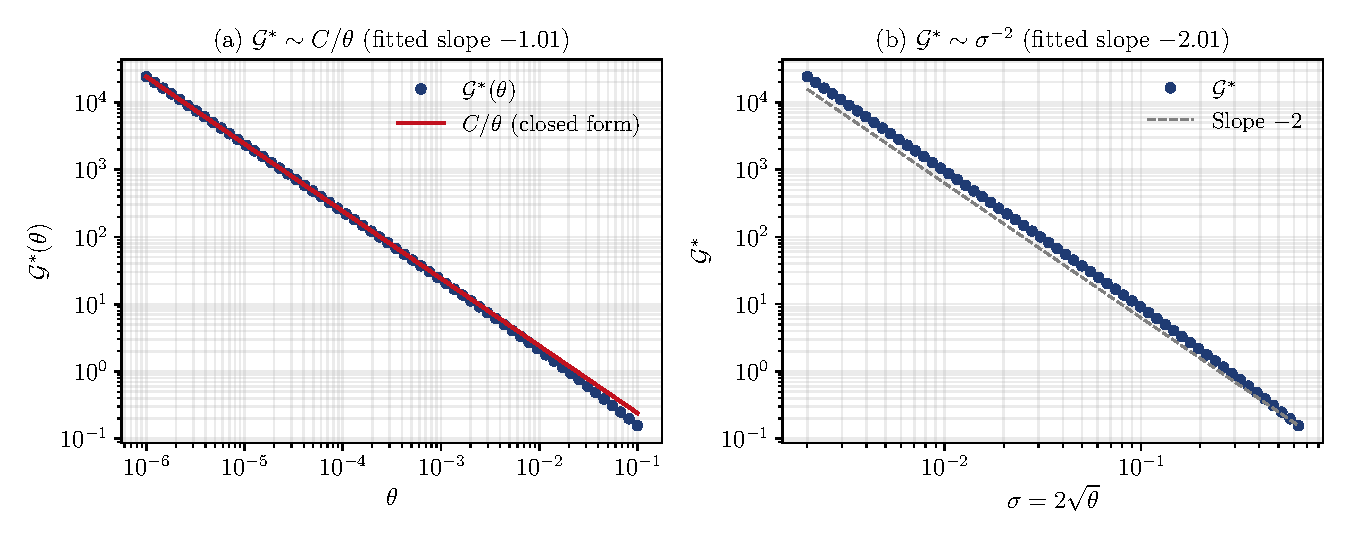
\includegraphics[width=\textwidth]{figures/scalar_fold.pdf}
\caption{The closed-form scalar fold of Example~\ref{ex:scalarfold}, verifying
Theorem~\ref{thm:fold}: the two-state QSD coupled through $a(u)=a_0+\alpha u$ with
$F(\theta,u)=u^{2}-\theta$, $u^{*}=\sqrt\theta$, $\sigma=2\sqrt\theta$.
\textbf{(a)} The closed-loop Fisher metric $\mathcal G^{*}(\theta)$ tracks the
closed-form leading term $C/\theta$ with
$C=\tfrac{\alpha^{2}}{4}\sum_s(\partial_a\nu_s)^2/\nu_s$ (at $a=a_0$) as
$\theta\to0$. \textbf{(b)} Equivalently $\mathcal G^{*}\sim\sigma^{-2}$ (fitted slope
$-2.01$ on the asymptotic window $\theta\le10^{-3}$, where the leading $C/\theta$ dominates
the $O(\theta^{-1/2})$ correction). Computed in \texttt{figures/scalar\_fold.py}.}
\label{fig:scalar-fold}
\end{figure}

\begin{remark}[Stratification interpretation]\label{rem:stratification}
The previous theorem is local. Globally, if the projection $\pi\colon\mathcal S\to
\Theta$ is proper on the region of interest and satisfies the standard
Thom--Boardman genericity assumptions~\cite{GolubitskyGuillemin1973}, its
discriminant $\mathcal B$ admits a Whitney
stratification~\cite{Whitney1965,Mather2012}: the regular values form open
\emph{regimes}, the $A_1$ fold points form the generic codimension-one walls, and
$A_2$ cusp points and higher singularities form higher-codimension strata. On each
regular regime, the closed-loop response geometry is analytic and bounded on
compact subsets. Approaching a fold wall along a regular branch, the local behavior
is the rank-one blow-up of Theorem~\ref{thm:fold}, subject to the
observable-coupling condition $\partial_u\nu\,e\neq0$ for the QSD metric and
$\partial_u\Lambda\,e\neq0$ for the rate channel. This is a global interpretation
of the local fold theorem under standard genericity hypotheses, not a separate
theorem proved here.
\end{remark}

\begin{remark}[Small-noise regularization]\label{rem:slowing}
When $F=0$ arises as the deterministic limit of an order-parameter diffusion
$\dd u=F(\theta,u)\,\dd t+\sigma_{\mathrm noise}\,\dd W$, the saddle--node normal
form along the fold direction fixes the regularized critical-layer width
$W\sim\sigma_{\mathrm noise}^{2/3}$ and relaxation time
$\tau\sim\sigma_{\mathrm noise}^{-2/3}$, so the leverage saturates at
$\sim\sigma_{\mathrm noise}^{-2/3}$ and recovers the divergence of
Theorem~\ref{thm:fold} as $\sigma_{\mathrm noise}\to0$; with
$\sigma_{\mathrm noise}^{2}\propto1/N$ these read $W\sim N^{-1/3}$,
$\tau\sim N^{1/3}$ \cite[Ch.~X]{vanKampen2007},\cite{Kuznetsov2004}. These are
the standard Fokker--Planck scaling heuristics, recorded for orientation only:
nothing in this paper depends on them, and they are not established here at the
rigor of \S\ref{sec:perturbation}.
\end{remark}


\section{Examples}\label{sec:examples}


\subsection{The two-state killed chain}\label{sec:two-state}

Let $T=\{1,2\}$ and
\[
Q=\begin{pmatrix}-(a+\kappa)&a\\ b&-b\end{pmatrix},
\qquad a,b>0,\ \kappa\ge0,
\]
killing $\kappa$ from state $1$ only, so $q=(\kappa,0)^{\top}$ and $Q$ is
irreducible iff $a,b>0$, properly killed iff $\kappa>0$.

\begin{example}[Closed-form principal datum and response]\label{ex:two-state}
The characteristic polynomial gives eigenvalues
$\lambda_{\pm}=\tfrac12\bigl[-(a+\kappa+b)\pm\sqrt{(a+\kappa-b)^{2}+4ab}\,\bigr]$,
and the principal datum is $-\Lambda=\lambda_{+}$:
\[
\Lambda=\tfrac12\Bigl[(a+\kappa+b)-\sqrt{(a+\kappa-b)^{2}+4ab}\Bigr]>0 .
\]
The left/right Perron vectors (normalized $\nu\one=1$, $\nu h=1$) are
\[
\nu\propto\bigl(b,\ a+\kappa-\Lambda\bigr),\qquad
h\propto\Bigl(1,\ \tfrac{b}{\,b-\Lambda\,}\Bigr),
\]
both strictly positive since $a+\kappa-\Lambda=\tfrac12[(a+\kappa-b)+\sqrt{(a+\kappa
-b)^2+4ab}]>0$ and $b-\Lambda=\tfrac12[-(a+\kappa-b)+\sqrt{(a+\kappa-b)^2+4ab}]>0$;
the two equivalent forms $h_2/h_1=(a+\kappa-\Lambda)/a=b/(b-\Lambda)$ coincide by
the characteristic identity $\Lambda^2-(a+\kappa+b)\Lambda+\kappa b=0$. The Hellmann--Feynman and reduced-resolvent
formulas \eqref{eq:dLambda}--\eqref{eq:dnu} reproduce $\partial\Lambda/\partial
a,\partial\Lambda/\partial\kappa$ and $\partial\nu/\partial a$ exactly; we verified
this symbolically and numerically. As $\kappa\to0$: $\Lambda\to0$, $h\to\one$,
$\nu\to\pi=(b,a)/(a+b)$, $R\to Q_0^{\#}$, and \eqref{eq:dnu} becomes the
conservative $\partial_a\pi_1=-b/(a+b)^2$ of Remark~\ref{rem:sign}, with the
positive sign $+\pi Q_aZ$.
\end{example}

\subsection{The scaling gauge and the channel split}

The two response coordinates $\nu$ and $\Lambda$ have genuinely different
kernels (Figure~\ref{fig:channel-split}). The cleanest witness is the overall
time-scaling symmetry, present in every family.

\begin{proposition}[Channel split]\label{prop:channel-split}
Let $s>0$ act on a sub-generator by $Q\mapsto sQ$. Then the principal datum
transforms as
\[
\nu(sQ)=\nu(Q),\qquad h(sQ)=h(Q),\qquad \Lambda(sQ)=s\,\Lambda(Q),\qquad R(sQ)=s^{-1}R(Q).
\]
Consequently, for any family containing a scaling direction
$\partial_{\log s}$ at $\theta$,
\[
\partial_{\log s}\nu=0
\quad\text{but}\quad
\partial_{\log s}\Lambda=\Lambda\neq0 .
\]
Hence $\partial_{\log s}\in\ker J=\ker\mathcal G$ but
$\partial_{\log s}\notin\ker\nabla\Lambda$: the distributional and rate channels of
Remark~\ref{rem:channels} have distinct kernels, and the augmented metric
$\mathcal G^{\oplus}$ of \eqref{eq:augmented} is strictly larger than $\mathcal G$
in the scaling direction.
\end{proposition}

\begin{proof}
$sQ$ has eigenvalues $s\,\spec(Q)$ with identical eigenvectors, so
$\Lambda(sQ)=s\Lambda(Q)$ and $\nu,h$ are unchanged; $R(sQ)=(sQ+s\Lambda
I)^{\#}=(s(Q+\Lambda I))^{\#}=s^{-1}(Q+\Lambda I)^{\#}=s^{-1}R$ by the scaling law of
the group inverse. Differentiating in $\log s$ at $s=1$ gives the displayed
derivatives, whence the kernel statements; $\mathcal G^{\oplus}-\mathcal
G=w\,\dd(\log\Lambda)^{\otimes2}$ evaluates to $w\neq0$ on $\partial_{\log s}$ since
$\partial_{\log s}\log\Lambda=1$.
\end{proof}

\begin{figure}[ht]
\centering
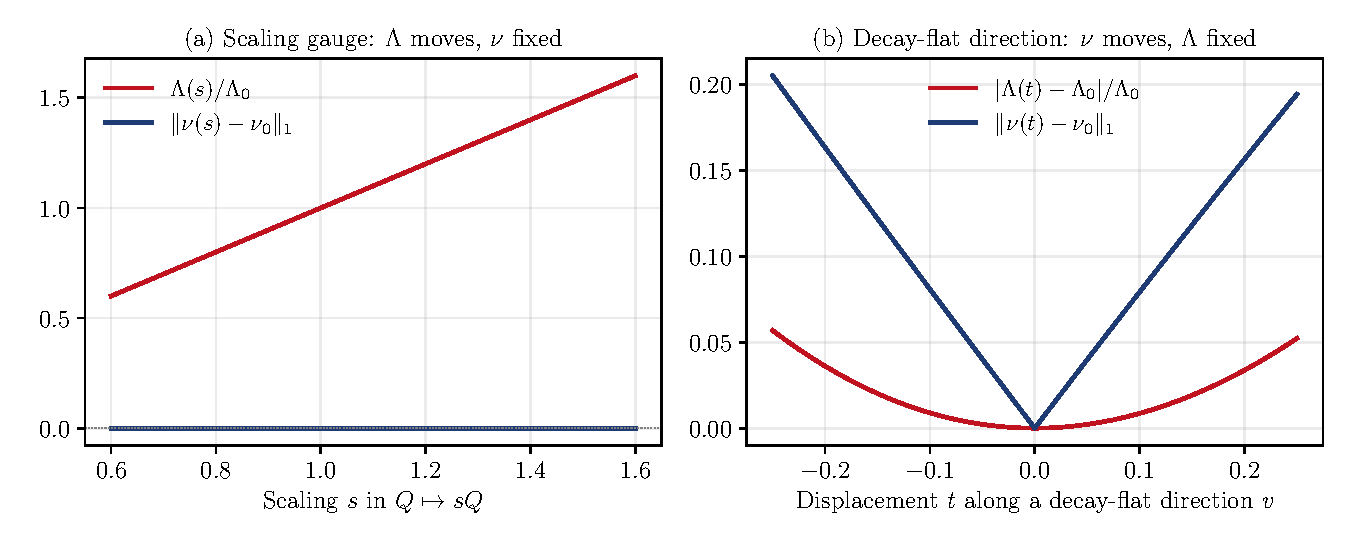
\includegraphics[width=\textwidth]{figures/channel_split.pdf}
\caption{The QSD and decay-rate channels are distinct
(Definition~\ref{def:augmented}, Proposition~\ref{prop:channel-split}), on the
two-state killed chain $Q(a,b,\kappa)$. \textbf{(a)} Along the scaling gauge
$Q\mapsto sQ$ the quasi-stationary distribution $\nu$ is exactly invariant
($\|\nu(s)-\nu_0\|_1=0$) while the decay rate scales linearly --- a perturbation in
$\ker J_\nu$ but not $\ker\nabla\Lambda$. \textbf{(b)} Along a direction in
$\ker\nabla\Lambda$, the decay rate is stationary to first order while $\nu$ moves
--- a perturbation in $\ker\nabla\Lambda$ but not $\ker J_\nu$. A perturbation may
thus move $\Lambda$ without moving $\nu$, or conversely. Computed in
\texttt{figures/channel\_split.py}.}
\label{fig:channel-split}
\end{figure}

\begin{remark}
Proposition~\ref{prop:channel-split} is the structural reason the decay rate is
worth carrying as a separate observable: it sees the overall time scale, to which
the conditional law $\nu$ is blind. More generally, any one-parameter group of
\emph{rate symmetries} of the family (gauge directions that rescale the generator
without changing its conditional law) lies in $\ker J$ but not in
$\ker\nabla\Lambda$, and produces an exact non-identifiability leaf
(Theorem~\ref{thm:rank}) for the distributional channel.
\end{remark}

\subsection{A self-consistent three-state fold}\label{sec:three-state}

\begin{example}[Fold-induced divergence]\label{ex:fold}
Let $T=\{1,2,3\}$ with a killed cycle whose activation rate is modulated by an
order parameter $u\in(0,1)$ through a sigmoidal feedback, e.g.
\[
Q(\theta,u)=
\begin{pmatrix}
-(\alpha(\theta,u)+\kappa_1) & \alpha(\theta,u) & 0\\
\beta & -(\beta+\gamma) & \gamma\\
\delta & 0 & -\delta
\end{pmatrix},
\quad
\alpha(\theta,u)=\alpha_0\,e^{\,g\,\varsigma(u-\theta)},
\]
with $\varsigma$ a smooth increasing saturating (sigmoidal) function and a single
small killing $\kappa_1>0$. Couple $u$ self-consistently to the activation prevalence by
$F(\theta,u)=\nu_1(\theta,u)-u$ \textup{(}or any analytic closure with
$\partial_uF$ changing sign\textup{)}. For a range of the gain $g$ the equation
$F=0$ has the S-shaped graph of a fold: two stable branches separated by a fold
locus $\mathcal B=\{\partial_uF=0\}$ in $\theta$. On each open regime
$\Theta\setminus\mathcal B$, Theorem~\ref{thm:fold} gives bounded analytic
closed-loop response; approaching $\mathcal B$, $\partial_\theta u^{*}$ diverges
rank-one, and --- since $\partial_u\nu$ couples to the fold here ---
$\dd\Phi^{*}$, $\nabla\Lambda^{*}$, $\mathcal G^{*}$ inherit it along the fold
direction, with the dominant eigenvector of $\mathcal G^{*}$ aligning with
$v_{*}\propto(\partial_\theta F)^{\top}\ell$. The univariate ($m=1$) case makes
$\ell=e=1$ and $\sigma=|\partial_uF|$, so $\partial_\theta u^{*}=-\partial_\theta
F/\partial_uF$ and the divergence is the textbook implicit-function blow-up at a
fold, here transported through $\nu$ and $\Lambda$ to the full information geometry.
This is the local model behind Remark~\ref{rem:stratification}: parameter space splits
into regimes of qualitatively distinct quasi-stationary behavior, separated by the
fold wall on which the response is maximally sensitive.

\smallskip
\noindent\emph{A verified instance.} Take $\varsigma=\tanh$ and the concrete
parameters
\[
(\beta,\gamma,\delta,\kappa_1,\alpha_0,g)=(1,\,0.8,\,1.2,\,0.05,\,1,\,-5).
\]
Since $\nu_1$ depends on $(\theta,u)$ only through $w:=u-\theta$, the equilibrium
branch is traced parametrically: with $G(w):=\nu_1\bigl(\alpha_0e^{g\varsigma(w)}\bigr)$
it is $\{(\theta,u)=(G(w)-w,\,G(w))\}$, and the fold condition $\partial_uF=0$
reads $G'(w)=1$. Here $\max_wG'(w)\approx1.24>1$, so two folds occur (at
$w\approx\pm0.18$) and the branch is bistable (Figure~\ref{fig:fold}(a)).
Approaching a fold along the branch, a direct computation from~\eqref{eq:dnu},
\eqref{eq:dLambda}, and the group inverse $R=(A+P)^{-1}(I-P)$ confirms the
predicted scalings: log--log regression of the response norms against
$\sigma=|\partial_uF|$ over three decades
($\sigma\in[\,2.3\times10^{-4},\,2.4\times10^{-1}\,]$) gives slopes
$-1.03$, $-1.03$, and $-2.03$
for $\|\dd\Phi^*\|$, $|\nabla\Lambda^*|$, and $\lambda_{\max}(\mathcal G^*)$
respectively, matching the predicted $-1,-1,-2$ of Theorem~\ref{thm:fold}
(Figure~\ref{fig:fold}(b)). The computation uses only the response calculus of
\S\ref{sec:perturbation} and is reproducible via the script
\texttt{figures/fold\_example.py}.
\end{example}

\begin{figure}[ht]
\centering
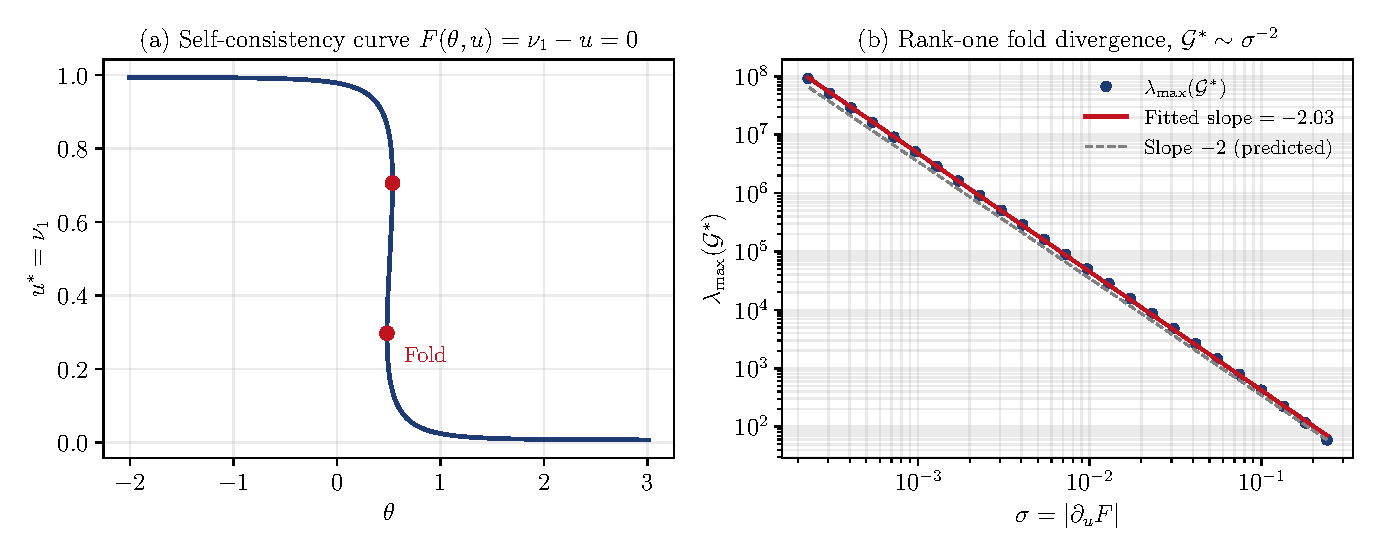
\includegraphics[width=\textwidth]{figures/fold_example.pdf}
\caption{Worked instance of the self-consistent three-state fold
(Example~\ref{ex:fold}), with $\varsigma=\tanh$ and
$(\beta,\gamma,\delta,\kappa_1,\alpha_0,g)=(1,0.8,1.2,0.05,1,-5)$.
\textbf{(a)} The self-consistency curve $F(\theta,u)=\nu_1(\theta,u)-u=0$ is
S-shaped; the two red dots are the folds $\partial_uF=0$ bounding the bistable
window. \textbf{(b)} Approaching a fold, the closed-loop Fisher metric diverges as
$\mathcal G^*\sim\sigma^{-2}$ in $\sigma=|\partial_uF|$ (fitted slope $-2.03$
against the predicted $-2$), the rank-one divergence of Theorem~\ref{thm:fold};
the norms $\|\dd\Phi^*\|$ and $|\nabla\Lambda^*|$ scale as $\sigma^{-1}$ (slopes
$-1.03$). Computed solely from the response formulas of \S\ref{sec:perturbation}.}
\label{fig:fold}
\end{figure}


\section{Infinite-dimensional generators}\label{sec:infinite-dim}

\emph{Status of this section.} The statements are split by proof obligation.
Proposition~\ref{thm:inf-exist} is a \emph{cited assembly}: under the standing hypotheses of
Assumption~\ref{ass:infinite}, cited operator theory (Champagnat--Villemonais, Krein--Rutman,
Meyn--Tweedie) yields the isolated simple principal eigentriple, the bounded reduced resolvent,
and the gap-as-conditional-ergodicity-rate identification. Proposition~\ref{thm:inf-response}
(the operator-valued derivative formulas) and Theorem~\ref{thm:inf-fold} (fold amplification
and the $\Lambda\to0$ recovery) are then \emph{conditional transport}: elementary deductions
from an isolated simple eigentriple and a bounded reduced resolvent, borrowing no further QSD
theory --- Theorem~\ref{thm:inf-fold}'s recovery carrying the additional gap-persistence
hypothesis stated there. Assumption~\ref{ass:infinite} is discharged concretely on the
exactly-solvable countable instance Example~\ref{ex:unbounded}. This is an \emph{assembly} of
cited theorems for the countable case, not a new theorem. Remark~\ref{rem:inf-diffusion} (the
diffusion case) is a roadmap at the rigor of a sketch and is \emph{not} part of the proved
package.

Everything above is finite-dimensional, where Perron--Frobenius supplies simplicity and the gap for
free. The natural objection is that the finite Metzler setting switches off every analytic difficulty
--- non-compactness, unboundedness, the principal eigenvalue merging into the essential spectrum ---
that makes infinite-dimensional QSD theory hard. This section lifts the response geometry to
non-compact state spaces, the missing ingredients supplied by a Foster--Lyapunov drift in place of
finite Perron--Frobenius; as the status note records, the countable case is a rigorous corollary
discharged on Example~\ref{ex:unbounded}, the diffusion case a sketch (Remark~\ref{rem:inf-diffusion}).
Companion proof notes, available with the source, hold the routine verifications.

\subsection{Setting and hypotheses}
Let $E$ be a Polish state space (countable discrete, or a domain in $\R^d$), $\partial$
an absorbing cemetery, and $(X_t)$ a $\mu$-irreducible Markov process on
$E\cup\{\partial\}$ with sub-Markovian generator $L$ on $E$ (an infinite Metzler
matrix in the discrete case; a second-order elliptic operator with killing potential
$\kappa\ge0$ in the diffusion case). The new feature is unboundedness: $L$ is
unbounded, $E$ is infinite, and there is no a priori spectral gap. The control object
is a \emph{Lyapunov (Foster) weight} $W\colon E\to[1,\infty)$ with $W\to\infty$ at
infinity, in whose weighted space $B_W=\{f:\|f\|_W:=\sup_x|f(x)|/W(x)<\infty\}$ the
spectral theory is recovered.

\begin{assumption}[Standing hypotheses]\label{ass:infinite}
\textup{(H1)} $P_t$ is irreducible and positivity-improving. \textup{(H2)} The
killing is accessible and not identically zero. \textup{(H3)} \emph{Foster--Lyapunov
drift:} there exist $W$ as above, constants $c>0$, $b<\infty$, and a small set
$K\subset E$ with $LW\le-cW+b\mathbf 1_K$ on $E$. \textup{(H4)} \emph{Doeblin
minorization on $K$:} there are $t_0>0$, $\theta>0$, and a probability $\nu_0$ with
$P_{t_0}(x,\cdot)\ge\theta\nu_0(\cdot)$ for all $x\in K$.
\end{assumption}

(H3)--(H4) are exactly the Champagnat--Villemonais conditions; (H1)--(H2) supply
irreducibility and a genuine killed process. The compact case is $W\equiv1$, $K=E$;
the finite-state case of \S\ref{sec:spectral} is $E$ finite, $W\equiv1$.

\begin{proposition}[QSD existence, simple isolated eigentriple, bounded reduced resolvent --- cited corollary]\label{thm:inf-exist}
This is an assembly of cited QSD theory, not a new deduction. Under
Assumption~\ref{ass:infinite} there is a unique quasi-stationary distribution $\nu$ on
$E$ and a principal eigentriple $(\Lambda,\nu,h)$ with $\Lambda>0$, $\nu L=-\Lambda\nu$,
$Lh=-\Lambda h$, $h\in B_W$, $h>0$, $\nu(h)=1$, such that $-\Lambda$ is a real,
algebraically simple, isolated eigenvalue of $L$ on $B_W$ with the rest of the spectrum
in $\{\Re z\le-\Lambda-g\}$ for a gap $g>0$; consequently the reduced resolvent
$R=(L+\Lambda I)^{\#}$ is bounded on $B_W$. The gap \emph{is} the conditional-ergodicity
rate: for every $\mu$ with $\mu(W)<\infty$,
$\|P_\mu(X_t\in\cdot\mid t<\tau_\partial)-\nu\|_{\mathrm{TV}}\le C(\mu)e^{-gt}$ with the
same $g$. The one genuinely nontrivial borrowed step is the passage from the Foster drift
\textup{(H3)} to a spectral gap for the \emph{sub-Markovian} (killed, not conservative)
semigroup $P_t$ on $B_W$: for the killed process this gap --- equivalently the exponential
conditional ergodicity below, together with existence and uniqueness of $\nu$ --- is supplied by the
Champagnat--Villemonais criterion \cite{ChampagnatVillemonais2016,ChampagnatVillemonais2017} (the
general weighted-space Foster--Lyapunov drift framework being Meyn--Tweedie \cite{MeynTweedie2009},
which is conservative), and the simple strictly positive principal eigenfunction is Krein--Rutman
\cite{KreinRutman1948}.
\end{proposition}

\begin{proposition}[Operator-valued response calculus --- conditional transport]\label{thm:inf-response}
\emph{Assume} an isolated, algebraically simple principal eigentriple $(\Lambda,\nu,h)$
with a bounded reduced resolvent $R=(L+\Lambda I)^{\#}$ on $B_W$ (as supplied by
Proposition~\ref{thm:inf-exist}), and that $L=L(p)$ is a holomorphic family of type
\textup{(A)} in a control $p$ (e.g.\ $\partial_pL$ relatively $L$-bounded). Then
$(\Lambda,\nu,h)$ are real-analytic in $p$ and
\[
\partial_p\Lambda=-\nu(\partial_pL)h,\qquad
\partial_p\nu=-\nu(\partial_pL)R+c_p\nu,\quad c_p=\nu(\partial_pL)R\mathbf 1,
\]
identical in form to the finite-state formulas of Theorem~\ref{thm:response}, with $R$
the group inverse of the unbounded generator on $B_W$. This is an elementary deduction
from the displayed hypotheses, conditional on them; it borrows no further QSD theory.
\end{proposition}

\begin{theorem}[Fold amplification and the $\Lambda\to0$ recovery]\label{thm:inf-fold}
On a stable self-consistent branch with slow eigenvalue $\sigma\to0$, the
finite-state amplification holds verbatim: $\partial_pu_*=F_p/\sigma$,
$\partial_p\Lambda=\Lambda'(u_*)F_p/\sigma+O(1)$, and the pulled-back Fisher metric
is $\Theta(\sigma^{-2})$, with the same observable-coupling condition. Moreover, if
the conservative generator $L_0$ (killing scaled to zero) is itself exponentially
ergodic in $B_W$ \emph{and, in addition, its weighted-space spectral gap persists under
the killing-scaling perturbation}, i.e.\ $\liminf_{\Lambda\to0}g(\Lambda)\ge g_0>0$, then as
$\kappa\downarrow0$ one has $\Lambda\to0$, $\nu\to\pi$, and
$R\to(L_0)^{\#}$ in operator norm:
the killed response calculus converges to the stationary
\textup{(}Schweitzer--Meyer\textup{)} calculus, the infinite-dimensional analogue of
Theorem~\ref{thm:conservative-limit}. (The gap-persistence hypothesis is automatic in finite
dimensions; in $B_W$ it is an assumption, not a conclusion --- see the proof.)
\end{theorem}

\begin{proof}
Proposition~\ref{thm:inf-exist} is the cited assembly under Assumption~\ref{ass:infinite};
Proposition~\ref{thm:inf-response} and Theorem~\ref{thm:inf-fold} are then elementary
deductions \emph{conditional on its conclusions} (an isolated simple eigentriple and a
bounded reduced resolvent). We give all three here (companion proof notes hold only the routine
verifications).
For the countable case the hypotheses (H1)--(H4) are moreover discharged concretely in
Example~\ref{ex:unbounded}, so the assembled eigentriple is realized, not merely conditional.

\emph{Proposition~\ref{thm:inf-exist}.} (H3)--(H4) are exactly the
Champagnat--Villemonais hypotheses
\cite{ChampagnatVillemonais2016,ChampagnatVillemonais2017}, which give existence and
uniqueness of the quasi-stationary distribution $\nu$ and exponential conditional
ergodicity $\|P_\mu(X_t\in\cdot\mid t<\tau_\partial)-\nu\|_{\mathrm{TV}}\le
C(\mu)e^{-gt}$ for every $\mu$ with $\mu(W)<\infty$ --- the killed-process spectral gap $g>0$ on
$B_W$. (Mechanistically the Foster drift (H3), $LW\le-cW+b\mathbf 1_K$, is what compactifies the
killed semigroup $P_t\colon B_W\to B_W$: outside the small set $K$ the drift contracts $W$, so $P_t$
maps the unit ball of $B_W$ into a relatively compact set up to an arbitrarily small tail; the general
weighted-space Foster--Lyapunov drift framework is Meyn--Tweedie \cite{MeynTweedie2009} in the
conservative case, and the sub-Markovian gap is the Champagnat--Villemonais content cited above.) By
(H1)--(H2) the resolvent is
positivity-improving on the cone of $W$-dominated nonnegative functions, so
Krein--Rutman \cite{KreinRutman1948} yields a simple, strictly positive principal
eigenfunction $h\in B_W$, $h>0$, with eigenvalue $-\Lambda$ ($\Lambda>0$ because the
killing is accessible and nonzero, (H2)) that is isolated from the rest of the
spectrum by a gap $g>0$ equal to the conditional-ergodicity rate. Normalizing
$\nu L=-\Lambda\nu$, $Lh=-\Lambda h$, $\nu(h)=1$ gives the principal eigentriple.

\emph{Proposition~\ref{thm:inf-response}.} Isolation and simplicity make the Riesz
projection $\Pi=h\otimes\nu$ rank-one and, since $\partial_pL$ is relatively
$L$-bounded, $L(p)$ is a holomorphic family of type (A) on $B_W$; Kato's theory of a
simple isolated eigenvalue \cite{Kato1995} then makes $(\Lambda,\nu,h)$ and $\Pi$
real-analytic in $p$. The reduced resolvent $R=(L+\Lambda I)^{\#}$ is bounded on
$B_W$ precisely because of the gap $g>0$. Differentiating $Lh=-\Lambda h$ and
$\nu L=-\Lambda\nu$ and projecting off $\Pi$ with $R$ reproduces, verbatim, the
finite-state computation of Theorem~\ref{thm:response}:
$\partial_p\Lambda=-\nu(\partial_pL)h$ and
$\partial_p\nu=-\nu(\partial_pL)R+c_p\nu$, $c_p=\nu(\partial_pL)R\mathbf 1$, all
finite because $R$ is bounded.

\emph{Theorem~\ref{thm:inf-fold}.} The amplification argument of \S\ref{sec:manifold}
used only the scalar implicit function theorem applied to the self-consistency
relation and the finiteness of $\partial_p\Lambda,\partial_p\nu$; both are now
available from Proposition~\ref{thm:inf-response}, so $\partial_pu_*=F_p/\sigma$,
$\partial_p\Lambda=\Lambda'(u_*)F_p/\sigma+O(1)$, and the pulled-back Fisher metric is
$\Theta(\sigma^{-2})$, with the same observable-coupling condition. For the
$\Lambda\to0$ recovery, scaling the killing $\kappa\downarrow0$ is an analytic
perturbation of the isolated simple eigenvalue $0$ of the conservative generator
$L_0$. We \emph{assume} the weighted-space spectral gap persists under this perturbation,
$\liminf_{\Lambda\to0}g(\Lambda)\ge g_0>0$ (the stated hypothesis): in finite dimensions this is
automatic by continuity of the simple isolated eigenvalue, but in $B_W$ the killing perturbation is
not relatively compact in general, so persistence of the gap is an assumption rather than a
consequence of ergodicity of $L_0$ alone. Under it, $\Lambda\to0$,
$\nu\to\pi$, $R\to(L_0)^{\#}$ in operator norm, giving the stationary (Schweitzer--Meyer) calculus,
the infinite-dimensional analogue of Theorem~\ref{thm:conservative-limit}.

\emph{Status.} For the countable case (H1)--(H4) are \emph{verified}, not merely assumed, on
Example~\ref{ex:unbounded}, so the corollary is realized; the diffusion case is the sketch of
Remark~\ref{rem:inf-diffusion}, and the further fold-\emph{sensing} residual (the functional-CLT step,
companion paper~\cite{SarkarFoldSensing}) is Remark~\ref{rem:inf-scope}.
\end{proof}

\begin{remark}[Diffusion extension --- roadmap, not a proved result]\label{rem:inf-diffusion}
Let $E\subseteq\R^d$ be a domain and $L=\tfrac12\nabla\cdot(a\nabla\,\cdot\,)+b\cdot\nabla-\kappa$
a uniformly elliptic second-order operator with killing potential $\kappa\ge0$,
$\kappa\not\equiv0$, on a weighted space $B_W$ with $W\to\infty$ at $\partial E$ and at
infinity. Suppose $\partial_pL$ is relatively $L$-bounded on $B_W$ and the Foster drift
(H3) and minorization (H4) hold for the killed diffusion. Then the conclusions of
Propositions~\textup{\ref{thm:inf-exist}},~\textup{\ref{thm:inf-response}} and Theorem~\textup{\ref{thm:inf-fold}} are \emph{expected} to hold for $L$, but
we do not establish them at the rigor of \S\S\ref{sec:spectral}--\ref{sec:manifold}: the open inputs
are
(i) the verification of (H3)--(H4) for the specific elliptic $L$ (standard for
confining drifts, e.g.\ Ornstein--Uhlenbeck with killing, but model-dependent), and
(ii) the control of the essential spectrum showing the principal eigenvalue is isolated
in $B_W$ and the group inverse bounded there. Both are classical
(Champagnat--Villemonais for (i); Agmon/weighted-space spectral theory for (ii)) but are
operator-theoretic verifications we record only in sketch
(in the companion proof notes); the countable case
(Propositions~\ref{thm:inf-exist},~\ref{thm:inf-response} and Theorem~\ref{thm:inf-fold}, Example~\ref{ex:unbounded}) is the
one carried out in full. We state this as a roadmap, not a proposition, precisely because (i)--(ii)
are not discharged here.
\end{remark}

\subsection{An explicit exactly-solvable instance}
The hard infinite-dimensional ingredient is the Foster--Lyapunov drift (H3) on a
genuinely non-compact space. We exhibit it explicitly.

\begin{example}[Birth--death-with-killing chain]\label{ex:unbounded}
Take the active-count $n\in\{0,1,2,\dots\}$ as a continuous-time chain with birth
$n\to n+1$ at constant rate $\beta$, death $n\to n-1$ at rate $\mu n$, and killing
$n\to\partial$ at rate $\kappa n$ (absorbing). The living generator is
$(Lf)(n)=\beta(f(n+1)-f(n))+\mu n(f(n-1)-f(n))-\kappa n f(n)$; each living row sums to
$-\kappa n$, so the QSD identity $\Lambda=-\nu L\mathbf 1=\kappa\,\mathbb E_\nu[N]$
holds exactly. For the weight $W(n)=e^{\gamma n}$,
\[
\frac{(LW)(n)}{W(n)}=\beta(e^{\gamma}-1)-n\bigl[\mu(1-e^{-\gamma})+\kappa\bigr],
\]
\emph{affine in $n$ with strictly negative slope} for every $\gamma>0$, so (H3) holds
with explicit $N_0=\lceil(\beta(e^\gamma-1)+c)/(\mu(1-e^{-\gamma})+\kappa)\rceil$,
$K=\{0,\dots,N_0-1\}$, and $b=\max_{n\in K}(D(n)+c)W(n)$. The remaining hypotheses are
immediate: the chain is irreducible and positivity-improving on $\{0,1,2,\dots\}$ (birth
and death connect adjacent states, $\beta,\mu>0$), giving (H1); the killing $\kappa n$
is accessible and not identically zero for $\kappa>0$, giving (H2); and (H4) is the
Doeblin minorization on the \emph{finite} set $K$, automatic for an irreducible chain.
Thus all of (H1)--(H4) are discharged \emph{concretely}, not assumed. The recovery rate
$\mu n$ grows without bound, so the chain ``comes down from infinity'' and
Proposition~\ref{thm:inf-exist} applies on this genuinely non-compact space. Because both
down-rates are linear in $n$, the instance is \emph{exactly solvable}: with
$\rho:=\beta/(\mu+\kappa)$,
\[
\nu=\mathrm{Poisson}(\rho),\qquad
\Lambda=\frac{\kappa\beta}{\mu+\kappa}=\kappa\rho,\qquad
\text{spectral gap}=\mu+\kappa,
\]
since the choice $\rho=\beta/(\mu+\kappa)$ makes the $m$-coefficient of the per-state
eigen-relation vanish (this is why Poisson is stationary) and the constant equals
$-\Lambda$. For the calibrated instance $(\beta,\mu,\kappa,\gamma,c)=(1,\tfrac12,
\tfrac1{10},1,1)$ one gets $N_0=7$, $b\approx94.7$, $\rho=\tfrac53$,
$\Lambda=\tfrac16$, gap $=\tfrac35$, and exponential moment $\sum_n\nu(n)e^{\gamma
n}=e^{\rho(e-1)}\approx17.53$; a deterministic truncation reproduces $\Lambda$ and
the gap to $10^{-15}$ and the identity $\Lambda=\kappa\,\mathbb E_\nu[N]$ to
$5\times10^{-15}$ (Figure~\ref{fig:unbounded}). The rational drift threshold
$\bar D(7)=-91/80\le-1$ and the exact $(\Lambda,\text{gap})$/eigen-identities are
rational and reproducible in \texttt{UnboundedLyapunovKernel.lean}.
\end{example}

\begin{figure}[ht]
\centering
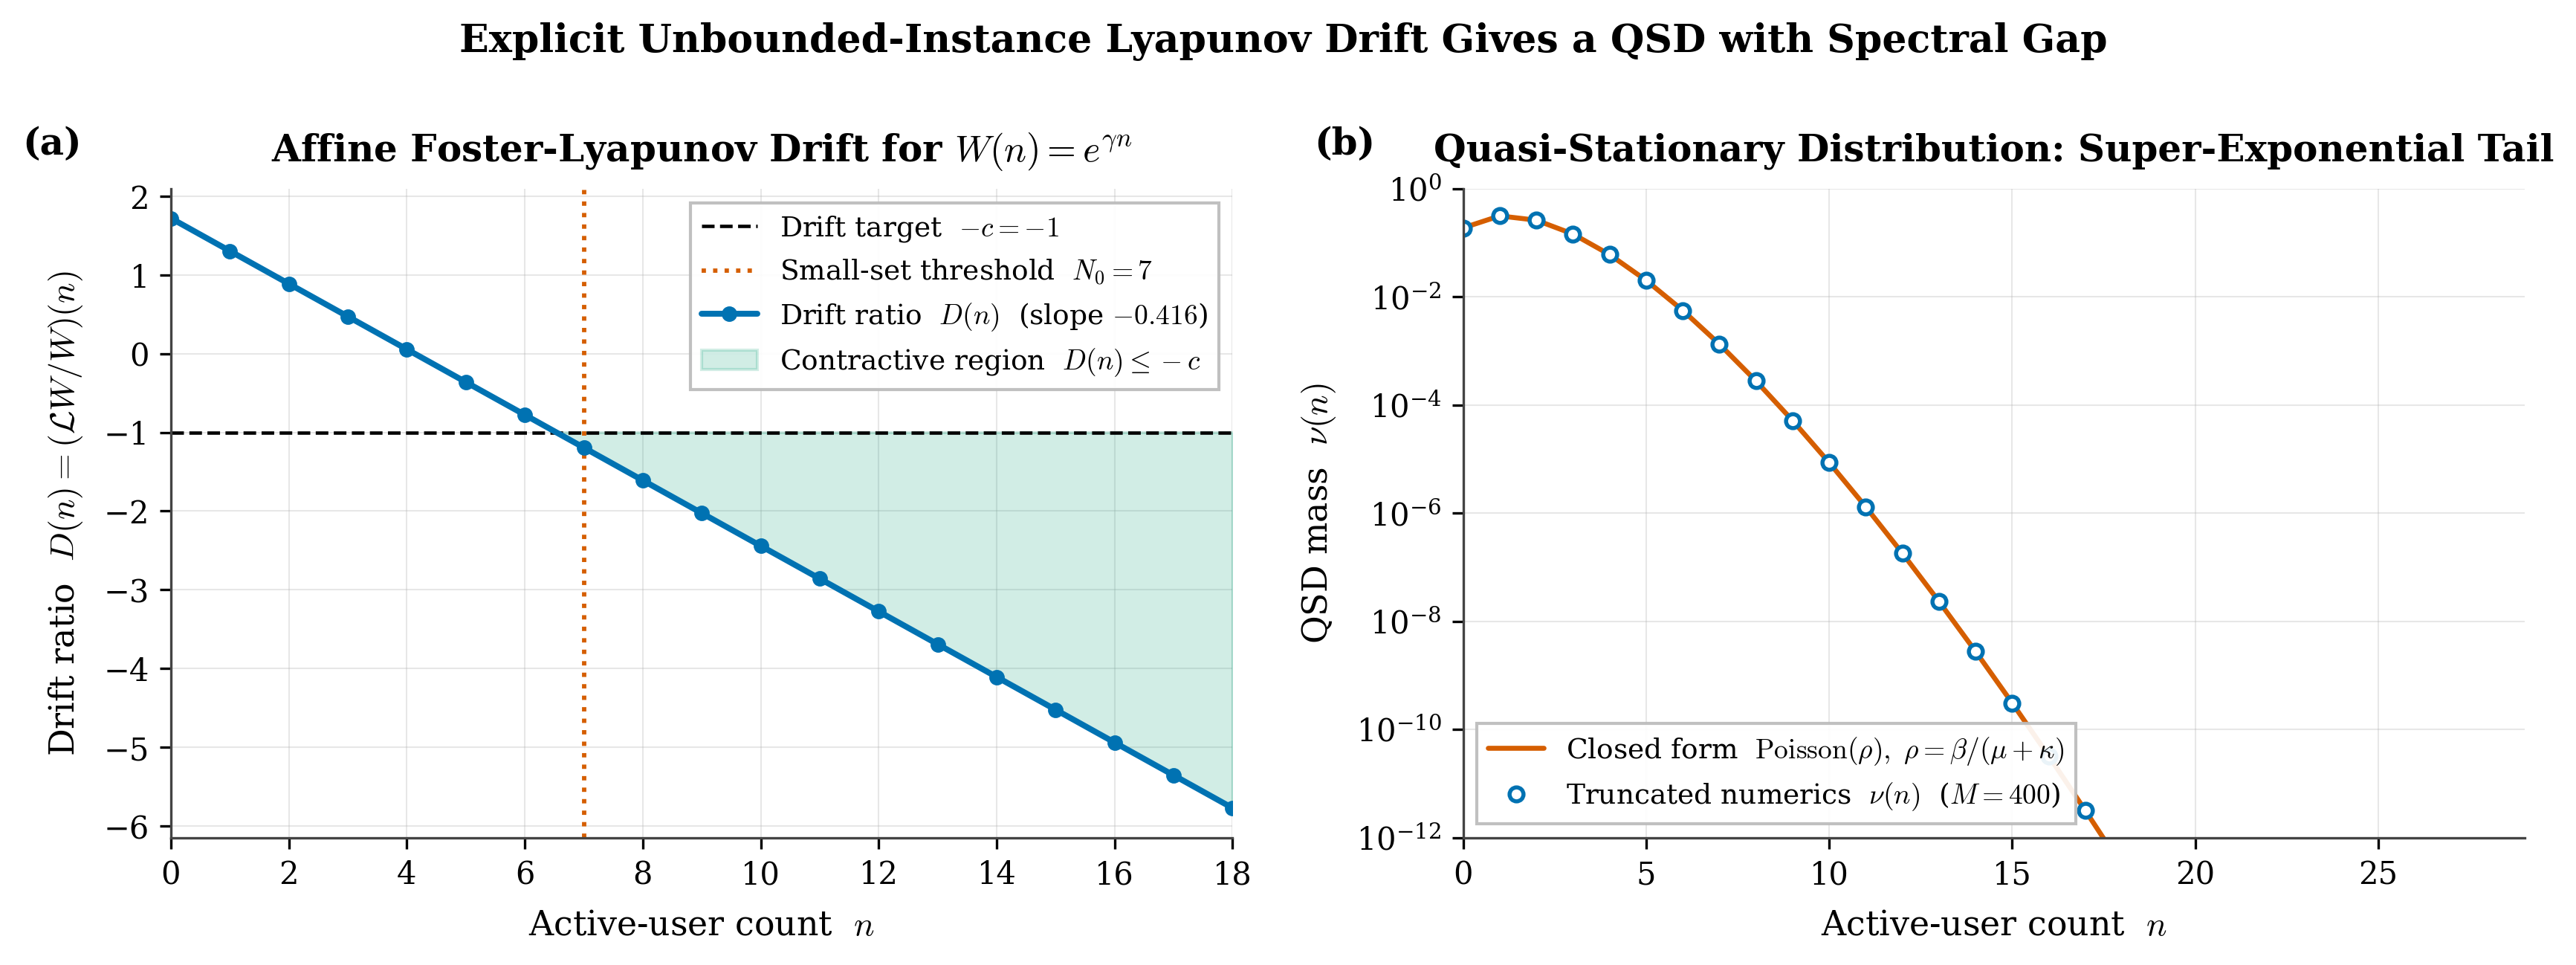
\includegraphics[width=\linewidth]{unbounded_qsd_lyapunov.png}
\caption{The explicit non-compact Foster--Lyapunov instance of
Example~\ref{ex:unbounded} (calibrated $(\beta,\mu,\kappa,\gamma)=(1,\tfrac12,
\tfrac1{10},1)$). \textbf{(left)} The drift ratio $D(n)=(LW/W)(n)$ for $W(n)=e^{\gamma
n}$ is affine in $n$ with strictly negative slope, crossing the level $-c=-1$ at
$N_0=7$; the shaded region marks $\{n\ge N_0\}$ where $D(n)\le-c$, certifying
$LW\le-cW+b\mathbf 1_K$ with the finite small set $K=\{0,\dots,6\}$. \textbf{(right)}
The resulting quasi-stationary distribution $\nu(n)$ (log scale) is
$\mathrm{Poisson}(\rho)$ with $\rho=\tfrac53$, exhibiting the super-exponential tail
that confines the chain on the unbounded state space. The exact $\Lambda=\tfrac16$
and gap $\tfrac35$ cross-check Proposition~\ref{thm:inf-exist} in closed form. Computed in
\texttt{analysis/unbounded\_qsd\_lyapunov.py}; rational core reproducible in
\texttt{UnboundedLyapunovKernel.lean}.}
\label{fig:unbounded}
\end{figure}

\begin{remark}[Scope of \S\ref{sec:infinite-dim}]\label{rem:inf-scope}
Two residuals lie beyond the countable assembly (whose status is the note opening this section; the
infinite-dimensional content over the finite case is that quasi-compactness, isolation, and the
bounded group inverse come from the Lyapunov drift rather than for free). The \emph{diffusion} case
(Remark~\ref{rem:inf-diffusion}) is at the rigor of a sketch, its open inputs the operator-theoretic
verification of (H1)--(H4) and the essential-spectrum control for elliptic $L$. The
infinite-dimensional \emph{fold-sensing} limit (companion paper~\cite{SarkarFoldSensing}) carries a
second: replacing the finite-$N$ demographic fluctuation by the functional-CLT fluctuation of the
empirical occupation measure is quantitative ($O(N^{-1/2})$) in the generic regime $\xi\gg1$, but on
the band $\xi=O(1)$ only a numerically checked generator-convergence with a $\sim N^{-2/3}$ error. The
finite-truncation algebraic kernel --- the group-inverse identity $(L+\Lambda I)R=I-h\otimes\nu$ and
the response formulas --- is reproducible in \texttt{InfiniteDimQSDKernel.lean} (exact on the
two-state instance; residuals $\le2\times10^{-10}$ on the model's $5\times5$ killed generator).
\end{remark}


\section{Concluding remarks}\label{sec:conclusion}


\subsection{Summary}
For a real-analytic family of irreducible Metzler sub-generators we have shown
that the principal spectral datum $(\Lambda,\nu)$ --- decay rate and
quasi-stationary distribution --- is real-analytic on the irreducible locus, that
its simplicity is rigid (Proposition~\ref{thm:rigidity}), and that its first-order
response is carried by the spectral projection and reduced resolvent
(Theorem~\ref{thm:response}). The QSD map endows parameter space with a canonical
Fisher information metric, equal to the pulled-back Fisher--Rao metric and the KL
Hessian, whose kernel is the non-identifiability foliation
(Theorems~\ref{thm:fisher},~\ref{thm:rank}); adjoining the decay rate adds a
rank-one rate channel (Definition~\ref{def:augmented}). Under a self-consistent
coupling the response acquires a rank-one singularity at simple folds, transmitted
to the QSD channel when $\partial_u\nu\,e\neq0$ and to the decay-rate channel when
$\partial_u\Lambda\,e\neq0$, and under genericity the discriminant carries a
stratified-regime interpretation
(Theorem~\ref{thm:fold} and Remark~\ref{rem:stratification}). The classical group-inverse
sensitivity theory of stationary distributions is the no-killing boundary case
(Theorem~\ref{thm:conservative-limit}).
Beyond the finite, noise-free core, the entire calculus lifts to non-compact countable
and diffusion state spaces, with an explicit exactly-solvable Foster--Lyapunov instance
(Propositions~\ref{thm:inf-exist},~\ref{thm:inf-response} and Theorem~\ref{thm:inf-fold}, Example~\ref{ex:unbounded}). The
companion paper~\cite{SarkarFoldSensing} carries the deterministic fold blow-up into the
finite-$N$ regime, where it is regularized by an exactly self-similar within-basin width
$W_N=(D/c)^{1/3}G(\xi)$, and shows that the $\sigma^{-2}$ amplification and the
finite-$N$ width are one object --- a fold-sensing resolution floor $R(\xi)=2G(\xi)/\xi$,
a Cram\'er--Rao bound on distance-to-fold estimation with a $\Theta(N^{-1/3})$ floor.

\subsection{The motivating application}\label{sec:applications}
The framework was distilled from a problem in mathematical epidemiology: a
finite-state model of a metastable behavioral population in which one state leaks
to an absorbing ``death'' state, so the long-run object is a quasi-stationary
distribution and a mortality-like decay rate. There, $\nu$ is the conditional
prevalence among survivors, $\Lambda$ the per-capita hazard, the parameters
$\theta$ are intervention-controllable rates, the information metric $\mathcal G$ is
an \emph{intervention-efficiency} tensor, its kernel encodes interventions with no
distributional effect, the self-consistent coupling is a mean-field prevalence
feedback whose fold is a tipping point, and the rank-one divergence is the outsized
leverage of interventions delivered near criticality. The \emph{channel split}
(Proposition~\ref{prop:channel-split}) there expresses that some interventions move
mortality without moving the conditional case-mix and conversely --- e.g.\ a
harm-reduction measure that lowers $\Lambda$ with little effect on $\nu$ versus an
enforcement measure transverse to both. We have deliberately stated the theory
with no such interpretation attached: it applies to any parametrized family of
killed finite Markov generators --- metastable chemical kinetics, reliability and
absorbing queueing models, population genetics with extinction, evolutionary
dynamics with absorbing fixation --- wherever the quasi-stationary datum is the
observable and its parameter dependence is the question.

\subsection{Extensions}
The infinite-state extension once listed here as future work is now carried out in
\S\ref{sec:infinite-dim}: for sub-Markovian generators on countable or continuous
state spaces with a Foster--Lyapunov drift, Kato's theory and the reduced-resolvent
calculus carry over to the operator setting, the rigidity supplied by Krein--Rutman
and quasi-compactness in place of finite Perron--Frobenius, with an explicit
exactly-solvable instance (Example~\ref{ex:unbounded}). Two further generalizations
remain. (1) \emph{Higher-order
information geometry}: the $\alpha$-connections and the dual-flat structure of the
response model invite a study of the embedding curvature of $\Phi(\Reg)$ in
$\Simp$, i.e.\ how far the QSD family is from an exponential family, and of the
$m$-projection estimator of Remark~\ref{rem:dually-flat} as a statistical
procedure. (2) \emph{Cusp and higher catastrophes}: Remark~\ref{rem:stratification}
isolates the fold as the generic wall, but cusps ($A_2$) and swallowtails ($A_3$)
appear in codimension and carry their own normal-form scalings for the response;
classifying the information-geometric signature of each elementary catastrophe is a
natural sequel.

\subsection*{Code availability}
{\sloppy
The source code (figure and verification scripts, the walkthrough notebook, and the Lean~4 kernels) is
available at the project repository
\textsf{[\textsc{repository url --- author to insert}]} and archived at
\textsf{[\textsc{Zenodo DOI --- author to mint}]}; the kernels and notebook are also bundled as arXiv
ancillary files.
All numerical claims in the paper are reproducible from the ancillary code:
\texttt{verify\_identities.py} checks every displayed first- and second-order
identity against central finite differences on randomly generated irreducible
Metzler families (Remark~\ref{rem:numerics});
\texttt{figures/fold\_example.py} regenerates the worked fold of
Example~\ref{ex:fold} (Figure~\ref{fig:fold}) and refuses to emit the figure
unless the fitted exponents match the predicted $(-1,-1,-2)$ within tolerance;
and a fully executed companion notebook
(\texttt{qsd\_response\_geometry\_walkthrough.ipynb}) restates each principal
result under its printed number and re-verifies it numerically. Every displayed
first- and second-order identity, including the right-eigenvector response
\eqref{eq:dh}, is checked in both the script and the notebook;
\texttt{analysis/eflat\_nonuniform\_qsd.py} verifies the $e$-flat non-uniform
construction of Example~\ref{ex:eflat-nonuniform} (exponential-family QSD, $h\neq\one$,
active $c_j$, and $\mathcal G=\operatorname{Cov}$) at $2\times10^{3}$ random points. No
external data are used.
The infinite-dimensional extension of \S\ref{sec:infinite-dim} is reproduced by
\texttt{analysis/\allowbreak unbounded\_qsd\_lyapunov.py} and
\texttt{analysis/\allowbreak infinite\_dim\_qsd\_kernel.py} (the non-compact instance and the
algebraic kernel, Figure~\ref{fig:unbounded}); the load-bearing rational identities
are machine-checked in the Lean~4~\cite{deMouraUllrich2021} kernels
\texttt{UnboundedLyapunovKernel.lean} and
\texttt{InfiniteDimQSDKernel.lean}, which ship self-contained in the companion subfolder
\texttt{lean/} with an executable walkthrough in \texttt{notebooks/}. The Lean layer verifies only
the \emph{rational core} over $\mathbb{Q}$---the group-inverse identity $(Q+\Lambda I)R=I-h\otimes\nu$
on the finite instance and Example~\ref{ex:unbounded}'s exactly-solvable Poisson QSD
($\Lambda=1/6$, gap $3/5$, $N_0=7$)---and \emph{not} the analytic Krein--Rutman/Kato content
on the weighted space, the infinite-dimensional limit, or Champagnat--Villemonais ergodicity,
which are cited; the per-kernel scope is in \texttt{lean/MAPPING.md} and the axiom profile in
\texttt{lean/AXIOMS.md}. The finite-$N$ and fold-sensing analysis
(\texttt{at\_fold\_*.py}, \texttt{fold\_sensing\_*.py}), the FLINT/Arb interval certificates
(continuum gap, variance band, and the new \emph{pending} discrete-gap certificate
\texttt{tools/cert\_discrete\_gap.py}), and the Agmon/Kato/discrete-Sturm rational kernels ship with
the companion paper~\cite{SarkarFoldSensing}.
\par}

\appendix


\section{The group inverse: existence, uniqueness, and the resolvent integral}\label{app:group}


For completeness we record the facts about the group inverse used above; see
\cite[Ch.~4]{CampbellMeyer2009},\cite{Meyer1975} for proofs.

\begin{lemma}\label{lem:group}
Let $A\in\R^{n\times n}$ have $0$ as a semisimple \textup{(}index-$1$\textup{)}
eigenvalue, so $\R^{n}=\ker A\oplus\Imm A$. Then there is a unique matrix
$A^{\#}$ with $AA^{\#}=A^{\#}A$, $A^{\#}AA^{\#}=A^{\#}$, $AA^{\#}A=A$; it acts as
$(A|_{\Imm A})^{-1}$ on $\Imm A$ and as $0$ on $\ker A$. If $P_0$ is the spectral
projection onto $\ker A$ along $\Imm A$, then $A^{\#}=(A+P_0)^{-1}(I-P_0)$ and
$AA^{\#}=I-P_0$. When $A=Q+\Lambda I$ for $Q\in\mathcal M_{\mathrm{irr}}(T)$ with
principal eigenvalue $-\Lambda$, the hypotheses hold with $P_0=P=h\nu$, giving the
reduced resolvent $R=A^{\#}$ of Definition~\ref{def:reduced-resolvent}, and the
contour representation
$R=\frac{1}{2\pi i}\oint_{\gamma}\frac{(zI-Q)^{-1}}{z+\Lambda}\,\dd z$,
$\gamma$ a small circle about $-\Lambda$ enclosing no other eigenvalue.
\end{lemma}

\begin{proof}
Existence/uniqueness and the projection formula are standard for index-$1$
matrices \cite[Thm.~4.5.2]{CampbellMeyer2009}. For the contour formula, the
resolvent has the Laurent expansion $(zI-Q)^{-1}=\dfrac{P}{z+\Lambda}+H(z)$ near
$z=-\Lambda$, where $P$ is the residue (the spectral projection) and $H$ is
holomorphic at $-\Lambda$ with $H(-\Lambda)=R$ the reduced resolvent (this is the
defining property of $R$ in Kato's Laurent expansion, no nilpotent part since the
eigenvalue is simple). Therefore
$\frac{(zI-Q)^{-1}}{z+\Lambda}=\frac{P}{(z+\Lambda)^{2}}+\frac{H(z)}{z+\Lambda}$,
whose residue at $z=-\Lambda$ is $0+H(-\Lambda)=R$; the contour integral equals this
residue by the residue theorem.
\end{proof}


\section{Kato analyticity for a simple isolated eigenvalue}\label{app:kato}


\begin{lemma}[{\cite[Ch.~II \S1.8, Ch.~VII \S1.3]{Kato1995}}]\label{lem:kato}
Let $\theta\mapsto A(\theta)\in\C^{n\times n}$ be real-analytic on an open set
$\Omega$, and suppose $A(\theta_0)$ has an algebraically simple eigenvalue
$\lambda_0$ isolated from the rest of the spectrum by a Jordan curve $\gamma$. Then
on a neighborhood of $\theta_0$ the Riesz projection
$P(\theta)=\frac{1}{2\pi i}\oint_{\gamma}(zI-A(\theta))^{-1}\,\dd z$ is real-analytic
and rank-one, the eigenvalue $\lambda(\theta)=\tr(A(\theta)P(\theta))$ is
real-analytic, and analytically normalized left/right eigenvectors exist. The
reduced resolvent $S(\theta)=\frac{1}{2\pi i}\oint_{\gamma}\frac{(zI-A)^{-1}}
{z-\lambda(\theta)}\,\dd z$ is real-analytic, and the first-order formulas
$\dd\lambda=\tr(P\,\dd A)$ and $\dd P=-(S\,\dd A\,P+P\,\dd A\,S)$ hold.
\end{lemma}

Applying Lemma~\ref{lem:kato} to $A=Q$, $\lambda_0=-\Lambda$, $S=R$ yields
Proposition~\ref{thm:rigidity}(i) and re-derives Theorem~\ref{thm:response}(a)--(b)
intrinsically; the simplex-normalized eigenvector formula
Theorem~\ref{thm:response}(c) is the additional content special to the
probability normalization $\nu\one=1$.


\begin{thebibliography}{99}

\bibitem{Amari2016} S.~Amari, \emph{Information Geometry and Its Applications},
Applied Mathematical Sciences \textbf{194}, Springer, Tokyo, 2016.

\bibitem{AmariNagaoka2000} S.~Amari and H.~Nagaoka, \emph{Methods of Information
Geometry}, Translations of Mathematical Monographs \textbf{191}, American
Mathematical Society, Providence, RI, 2000.

\bibitem{Arnold1992} V.~I.~Arnold, \emph{Catastrophe Theory}, 3rd ed., Springer,
Berlin, 1992.

\bibitem{Ay2017} N.~Ay, J.~Jost, H.~V.~L\^e, and L.~Schwachh\"ofer,
\emph{Information Geometry}, Ergebnisse der Mathematik und ihrer Grenzgebiete
\textbf{64}, Springer, Cham, 2017.

\bibitem{BerglundGentz2006} N.~Berglund and B.~Gentz, \emph{Noise-Induced
Phenomena in Slow--Fast Dynamical Systems: A Sample-Paths Approach}, Probability and
Its Applications, Springer, London, 2006.

\bibitem{BermanPlemmons1994} A.~Berman and R.~J.~Plemmons, \emph{Nonnegative
Matrices in the Mathematical Sciences}, Classics in Applied Mathematics \textbf{9},
SIAM, Philadelphia, 1994.

\bibitem{Bukten2017} A.~Bukten, S.~Stavseth, S.~Skurtveit, A.~Tverdal,
J.~R\o{}islien, and T.~Clausen, \emph{High risk of overdose death following release
from prison: variations in mortality during a 15-year observation period}, Addiction
\textbf{112} (2017), no.~8, 1432--1439.

\bibitem{ChampagnatVillemonais2016} N.~Champagnat and D.~Villemonais,
\emph{Exponential convergence to quasi-stationary distribution and $Q$-process},
Probab.\ Theory Related Fields \textbf{164} (2016), 243--283.

\bibitem{ChampagnatVillemonais2017} N.~Champagnat and D.~Villemonais,
\emph{General criteria for the study of quasi-stationarity}, Electron.\ J.\ Probab.\
\textbf{28} (2023), paper no.~22, 84 pp., DOI 10.1214/22-EJP880; arXiv:1712.08092.

\bibitem{CampbellMeyer2009} S.~L.~Campbell and C.~D.~Meyer, \emph{Generalized
Inverses of Linear Transformations}, Classics in Applied Mathematics \textbf{56},
SIAM, Philadelphia, 2009.

\bibitem{Cencov1982} N.~N.~\v{C}encov, \emph{Statistical Decision Rules and Optimal
Inference}, Translations of Mathematical Monographs \textbf{53}, American
Mathematical Society, Providence, RI, 1982.

\bibitem{ChoMeyer2001} G.~E.~Cho and C.~D.~Meyer, \emph{Comparison of perturbation
bounds for the stationary distribution of a Markov chain}, Linear Algebra Appl.
\textbf{335} (2001), 137--150.

\bibitem{ColletMartinezSanMartin2013} P.~Collet, S.~Mart\'inez, and J.~San
Mart\'in, \emph{Quasi-Stationary Distributions: Markov Chains, Diffusions and
Dynamical Systems}, Probability and Its Applications, Springer, Berlin, 2013.

\bibitem{DarrochSeneta1967} J.~N.~Darroch and E.~Seneta, \emph{On
quasi-stationary distributions in absorbing continuous-time finite Markov chains},
J. Appl. Probab. \textbf{4} (1967), 192--196.

\bibitem{DeutschNeumann1984} E.~Deutsch and M.~Neumann, \emph{Derivatives of the
Perron root at an essentially nonnegative matrix and the group inverse of an
M-matrix}, J. Math. Anal. Appl. \textbf{102} (1984), 1--29.

\bibitem{GolubMeyer1986} G.~H.~Golub and C.~D.~Meyer, \emph{Using the QR
factorization and group inversion to compute, differentiate, and estimate the
sensitivity of stationary probabilities for Markov chains}, SIAM J. Algebraic
Discrete Methods \textbf{7} (1986), 273--281.

\bibitem{GolubitskyGuillemin1973} M.~Golubitsky and V.~Guillemin, \emph{Stable
Mappings and Their Singularities}, Graduate Texts in Mathematics \textbf{14},
Springer, New York, 1973.

\bibitem{GoreskyMacPherson1988} M.~Goresky and R.~MacPherson, \emph{Stratified
Morse Theory}, Ergebnisse der Mathematik und ihrer Grenzgebiete \textbf{14},
Springer, Berlin, 1988.

\bibitem{GuckenheimerHolmes1983} J.~Guckenheimer and P.~Holmes, \emph{Nonlinear
Oscillations, Dynamical Systems, and Bifurcations of Vector Fields}, Applied
Mathematical Sciences \textbf{42}, Springer, New York, 1983.

\bibitem{HornJohnson2013} R.~A.~Horn and C.~R.~Johnson, \emph{Matrix Analysis},
2nd ed., Cambridge University Press, Cambridge, 2013.

\bibitem{JankeJohnstonKenna2004} W.~Janke, D.~A.~Johnston, and R.~Kenna,
\emph{Information geometry and phase transitions}, Phys. A \textbf{336} (2004),
181--186.

\bibitem{Kato1995} T.~Kato, \emph{Perturbation Theory for Linear Operators},
reprint of the 1980 ed., Classics in Mathematics, Springer, Berlin, 1995.

\bibitem{AbsIG2026} M.~Kimura, \emph{Information geometry of absorbing
Markov-chain and discriminative random walks}, Inf.\ Geom.\ (2026),
DOI 10.1007/s41884-026-00198-3, arXiv:2602.08185.

\bibitem{KrantzParks2013} S.~G.~Krantz and H.~R.~Parks, \emph{The Implicit
Function Theorem: History, Theory, and Applications}, Modern Birkh\"auser
Classics, Birkh\"auser, New York, 2013.

\bibitem{KreinRutman1948} M.~G.~Krein and M.~A.~Rutman, \emph{Linear operators
leaving invariant a cone in a Banach space}, Uspekhi Mat. Nauk \textbf{3} (1948),
no.~1, 3--95; English transl., Amer. Math. Soc. Transl. \textbf{26} (1950).

\bibitem{Kuznetsov2004} Yu.~A.~Kuznetsov, \emph{Elements of Applied Bifurcation
Theory}, 3rd ed., Applied Mathematical Sciences \textbf{112}, Springer, New York,
2004.

\bibitem{Lee2013} J.~M.~Lee, \emph{Introduction to Smooth Manifolds}, 2nd ed.,
Graduate Texts in Mathematics \textbf{218}, Springer, New York, 2013.

\bibitem{ModelManifoldGeom} D.~Lill, J.~Timmer, and D.~Kaschek, \emph{Local
Riemannian geometry of model manifolds and its implications for practical
parameter identifiability}, PLoS ONE \textbf{14} (2019), no.~6, e0217837,
DOI 10.1371/journal.pone.0217837.

\bibitem{Mather2012} J.~Mather, \emph{Notes on topological stability}, Bull. Amer.
Math. Soc. (N.S.) \textbf{49} (2012), 475--506.

\bibitem{MeleardVillemonais2012} S.~M\'el\'eard and D.~Villemonais,
\emph{Quasi-stationary distributions and population processes}, Probab. Surv.
\textbf{9} (2012), 340--410.

\bibitem{Meyer1975} C.~D.~Meyer, \emph{The role of the group generalized inverse in
the theory of finite Markov chains}, SIAM Rev. \textbf{17} (1975), 443--464.

\bibitem{MeynTweedie2009} S.~Meyn and R.~L.~Tweedie, \emph{Markov Chains and
Stochastic Stability}, 2nd ed., Cambridge University Press, Cambridge, 2009.


\bibitem{Prokopenko2011} M.~Prokopenko, J.~T.~Lizier, O.~Obst, and X.~R.~Wang,
\emph{Relating Fisher information to order parameters}, Phys. Rev. E \textbf{84}
(2011), 041116.

\bibitem{RudolfWang2021} D.~Rudolf and A.~Q.~Wang, \emph{Perturbation theory for
killed Markov processes and quasi-stationary distributions}, Adv.\ Appl.\ Probab.\
\textbf{57} (2025), no.~3, 1138--1165, DOI 10.1017/apr.2025.3.

\bibitem{SarkarFoldSensing} A.~Sarkar, \emph{A self-similar quasi-stationary width at a
saddle--node fold, and a finite-$N$ resolution floor for distance-to-criticality},
companion paper, in preparation (2026).

\bibitem{Schweitzer1968} P.~J.~Schweitzer, \emph{Perturbation theory and finite
Markov chains}, J. Appl. Probab. \textbf{5} (1968), 401--413.

\bibitem{Seneta2006} E.~Seneta, \emph{Non-negative Matrices and Markov Chains},
revised reprint, Springer Series in Statistics, Springer, New York, 2006.

\bibitem{Thom1969} R.~Thom, \emph{Ensembles et morphismes stratifi\'es}, Bull.
Amer. Math. Soc. \textbf{75} (1969), 240--284.

\bibitem{Transtrum2015} M.~K.~Transtrum, B.~B.~Machta, K.~S.~Brown, B.~C.~Daniels,
C.~R.~Myers, and J.~P.~Sethna, \emph{Perspective: Sloppiness and emergent theories
in physics, biology, and beyond}, J.\ Chem.\ Phys.\ \textbf{143} (2015), 010901.

\bibitem{vanDoornPollett2013} E.~A.~van Doorn and P.~K.~Pollett,
\emph{Quasi-stationary distributions for discrete-state models}, European J. Oper.
Res. \textbf{230} (2013), 1--14.

\bibitem{vanKampen2007} N.~G.~van Kampen, \emph{Stochastic Processes in Physics and
Chemistry}, 3rd ed., North-Holland, Amsterdam, 2007.

\bibitem{Whitney1965} H.~Whitney, \emph{Tangents to an analytic variety}, Ann. of
Math. (2) \textbf{81} (1965), 496--549.

\bibitem{deMouraUllrich2021} L.~de Moura and S.~Ullrich, \emph{The Lean~4 theorem prover and
programming language}, in Automated Deduction --- CADE-28, Lecture Notes in Computer Science
\textbf{12699}, Springer, 2021, pp.~625--635.

\end{thebibliography}

\end{document}
